% Options for packages loaded elsewhere
\PassOptionsToPackage{unicode}{hyperref}
\PassOptionsToPackage{hyphens}{url}
\PassOptionsToPackage{dvipsnames,svgnames,x11names}{xcolor}
%
\documentclass[a4paper,12pt]{article}
\usepackage[notransparent]{svg}
\usepackage[utf8]{inputenc}
\usepackage[lmargin=3cm,tmargin=3cm,rmargin=2cm,bmargin=2cm]{geometry}
\usepackage{fancyhdr}
\fancyhf{}
\fancyhead[R]{\thepage}
\renewcommand{\headrulewidth}{0pt}
\usepackage[onehalfspacing]{setspace}
\usepackage{blindtext}
\usepackage[T1]{fontenc}
% \usepackage[brazil]{babel}
\usepackage[document]{ragged2e}
\usepackage{pdflscape}
\usepackage{pdfpages}
\usepackage{float}
\usepackage{changepage}

\usepackage{graphicx, xcolor, comment, enumerate, multirow, multicol}
\usepackage{indentfirst}

\usepackage{amsfonts, amsthm, amsmath, amssymb, dsfont, mathtools}
\usepackage{tikz, tkz-base, tkz-fct}
\usepackage[style=abnt]{biblatex}

\usepackage{titlesec}
\usepackage{adjustbox}
\usepackage[skip=5pt, indent=15pt]{parskip}

\titleformat{\section}
{\normalsize\bfseries}{\thesection.}{1em}{}
\titleformat{\subsection}
{\normalsize}{\thesubsection.}{1em}{}
\titleformat{\subsubsection}
{\normalsize}{\thesubsubsection.}{1em}{}

\newcommand{\PR}[1]{\ensuremath{\left[#1\right]}}
\newcommand{\PC}[1]{\ensuremath{\left(#1\right)}}
\newcommand{\chav}[1]{\ensuremath{\left\{#1\right\}}}
\newcommand{\system}[1]{\ensuremath{\left\{#1\right}}
\newcommand{\floor}[1]{\ensuremath{\left \lfloor #1\right \rfloor}}
\newcommand{\FontTable}[1]{\vspace{-\baselineskip}\begin{footnotesize}#1\end{footnotesize}}

% Citacao direta com mais de 3 linhas - ABNT NBR 10520/2002 - 5.3
\newlength{\ABNTEXcitacaorecuo}% recuo de 4 cm da margem esquerda
\setlength{\ABNTEXcitacaorecuo}{4cm}
\newcommand{\ABNTEXfontereduzida}{\footnotesize}
\newenvironment*{citacao}[1][default]{%
   \list{}%
   \ABNTEXfontereduzida%
   \addtolength{\leftskip}{\ABNTEXcitacaorecuo}%
   \item[]%
   \singlespacing
   \ifthenelse{\not\equal{#1}{default}}{\itshape\selectlanguage{#1}}{}%
 }{%
   \endlist}%
% ---


% Citacao direta com mais de 3 linhas - ABNT NBR 10520/2002 - 5.3
\newlength{\aprovacao}% recuo de 4 cm da margem esquerda
\setlength{\aprovacao}{10.5cm}
\newcommand{\aprovacaofonte}{\normalsize}
\newenvironment*{citacao2}[1][default]{%
   \list{}%
   \aprovacaofonte%
   \addtolength{\leftskip}{\aprovacao}%
   \item[]%
   \singlespacing
   \justify
   \ifthenelse{\not\equal{#1}{default}}{\itshape\selectlanguage{#1}}{}%
 }{%
   \endlist}%
% ---


\newcommand{\fig}[4]{%
  \begin{figure}[H]
    \centering
    \caption{#1}
    \label{#2}
    \includegraphics{#3}
    
    \vspace{0.5cm}
    
    \begin{footnotesize}
      Fonte: #4
    \end{footnotesize}
  \end{figure}
}

\newcommand{\quadro}[4]{%
  \renewcommand{\figurename}{Quadro}
  \setcounter{figure}{0}
  \begin{figure}[H]
    \captionsetup{list=no}
    \centering
    \caption{#1}
    \label{#2}
    \includegraphics{#3}
    
    \vspace{0.5cm}
    
    \begin{footnotesize}
      Fonte: #4
    \end{footnotesize}
  \end{figure}
}

\newenvironment{invisible}{\color{white}}{}

\usepackage{amsmath,amssymb}
\usepackage{iftex}
\ifPDFTeX
  \usepackage[T1]{fontenc}
  \usepackage[utf8]{inputenc}
  \usepackage{textcomp} % provide euro and other symbols
\else % if luatex or xetex
  \usepackage{unicode-math}
  \defaultfontfeatures{Scale=MatchLowercase}
  \defaultfontfeatures[\rmfamily]{Ligatures=TeX,Scale=1}
\fi
\usepackage{lmodern}
\ifPDFTeX\else  
    % xetex/luatex font selection
  \setmainfont[]{Times New Roman}
\fi
% Use upquote if available, for straight quotes in verbatim environments
\IfFileExists{upquote.sty}{\usepackage{upquote}}{}
\IfFileExists{microtype.sty}{% use microtype if available
  \usepackage[]{microtype}
  \UseMicrotypeSet[protrusion]{basicmath} % disable protrusion for tt fonts
}{}
\makeatletter
\@ifundefined{KOMAClassName}{% if non-KOMA class
  \IfFileExists{parskip.sty}{%
    \usepackage{parskip}
  }{% else
    \setlength{\parindent}{0pt}
    \setlength{\parskip}{6pt plus 2pt minus 1pt}}
}{% if KOMA class
  \KOMAoptions{parskip=half}}
\makeatother
\usepackage{xcolor}
\setlength{\emergencystretch}{3em} % prevent overfull lines
\setcounter{secnumdepth}{5}
% Make \paragraph and \subparagraph free-standing
\ifx\paragraph\undefined\else
  \let\oldparagraph\paragraph
  \renewcommand{\paragraph}[1]{\oldparagraph{#1}\mbox{}}
\fi
\ifx\subparagraph\undefined\else
  \let\oldsubparagraph\subparagraph
  \renewcommand{\subparagraph}[1]{\oldsubparagraph{#1}\mbox{}}
\fi


\providecommand{\tightlist}{%
  \setlength{\itemsep}{0pt}\setlength{\parskip}{0pt}}\usepackage{longtable,booktabs,array}
\usepackage{calc} % for calculating minipage widths
% Correct order of tables after \paragraph or \subparagraph
\usepackage{etoolbox}
\makeatletter
\patchcmd\longtable{\par}{\if@noskipsec\mbox{}\fi\par}{}{}
\makeatother
% Allow footnotes in longtable head/foot
\IfFileExists{footnotehyper.sty}{\usepackage{footnotehyper}}{\usepackage{footnote}}
\makesavenoteenv{longtable}
\usepackage{graphicx}
\makeatletter
\def\maxwidth{\ifdim\Gin@nat@width>\linewidth\linewidth\else\Gin@nat@width\fi}
\def\maxheight{\ifdim\Gin@nat@height>\textheight\textheight\else\Gin@nat@height\fi}
\makeatother
% Scale images if necessary, so that they will not overflow the page
% margins by default, and it is still possible to overwrite the defaults
% using explicit options in \includegraphics[width, height, ...]{}
\setkeys{Gin}{width=\maxwidth,height=\maxheight,keepaspectratio}
% Set default figure placement to htbp
\makeatletter
\def\fps@figure{htbp}
\makeatother
\newlength{\cslhangindent}
\setlength{\cslhangindent}{1.5em}
\newlength{\csllabelwidth}
\setlength{\csllabelwidth}{3em}
\newlength{\cslentryspacingunit} % times entry-spacing
\setlength{\cslentryspacingunit}{\parskip}
\newenvironment{CSLReferences}[2] % #1 hanging-ident, #2 entry spacing
 {% don't indent paragraphs
  \setlength{\parindent}{0pt}
  % turn on hanging indent if param 1 is 1
  \ifodd #1
  \let\oldpar\par
  \def\par{\hangindent=\cslhangindent\oldpar}
  \fi
  % set entry spacing
  \setlength{\parskip}{#2\cslentryspacingunit}
 }%
 {}
\usepackage{calc}
\newcommand{\CSLBlock}[1]{#1\hfill\break}
\newcommand{\CSLLeftMargin}[1]{\parbox[t]{\csllabelwidth}{#1}}
\newcommand{\CSLRightInline}[1]{\parbox[t]{\linewidth - \csllabelwidth}{#1}\break}
\newcommand{\CSLIndent}[1]{\hspace{\cslhangindent}#1}

\makeatletter
\makeatother
\makeatletter
\makeatother
\makeatletter
\@ifpackageloaded{caption}{}{\usepackage{caption}}
\AtBeginDocument{%
\ifdefined\contentsname
  \renewcommand*\contentsname{Índice}
\else
  \newcommand\contentsname{Índice}
\fi
\ifdefined\listfigurename
  \renewcommand*\listfigurename{Lista de Figuras}
\else
  \newcommand\listfigurename{Lista de Figuras}
\fi
\ifdefined\listtablename
  \renewcommand*\listtablename{Lista de Tabelas}
\else
  \newcommand\listtablename{Lista de Tabelas}
\fi
\ifdefined\figurename
  \renewcommand*\figurename{Figura}
\else
  \newcommand\figurename{Figura}
\fi
\ifdefined\tablename
  \renewcommand*\tablename{Tabela}
\else
  \newcommand\tablename{Tabela}
\fi
}
\@ifpackageloaded{float}{}{\usepackage{float}}
\floatstyle{ruled}
\@ifundefined{c@chapter}{\newfloat{codelisting}{h}{lop}}{\newfloat{codelisting}{h}{lop}[chapter]}
\floatname{codelisting}{Listagem}
\newcommand*\listoflistings{\listof{codelisting}{Lista de Listagens}}
\makeatother
\makeatletter
\@ifpackageloaded{caption}{}{\usepackage{caption}}
\@ifpackageloaded{subcaption}{}{\usepackage{subcaption}}
\makeatother
\makeatletter
\makeatother
\ifLuaTeX
\usepackage[bidi=basic]{babel}
\else
\usepackage[bidi=default]{babel}
\fi
\babelprovide[main,import]{brazilian}
% get rid of language-specific shorthands (see #6817):
\let\LanguageShortHands\languageshorthands
\def\languageshorthands#1{}
\ifLuaTeX
  \usepackage{selnolig}  % disable illegal ligatures
\fi
\IfFileExists{bookmark.sty}{\usepackage{bookmark}}{\usepackage{hyperref}}
\IfFileExists{xurl.sty}{\usepackage{xurl}}{} % add URL line breaks if available
\urlstyle{same} % disable monospaced font for URLs
\hypersetup{
  pdftitle={AS CENTRALIDADES FINANCEIRAS NO ESPAÇO URBANO: UMA ANÁLISE ESPACIAL DO SETOR BANCÁRIO NO MUNICÍPIO DE SÃO PAULO.},
  pdfauthor={Flávio Hugo Pangracio Silva},
  pdflang={pt-BR},
  pdfkeywords={Centralidade; Sistema Financeiro; Economia Regional e
Urbana.},
  colorlinks=true,
  linkcolor={black},
  filecolor={Maroon},
  citecolor={Blue},
  urlcolor={Blue},
  pdfcreator={LaTeX via pandoc}}

\title{AS CENTRALIDADES FINANCEIRAS NO ESPAÇO URBANO: UMA ANÁLISE
ESPACIAL DO SETOR BANCÁRIO NO MUNICÍPIO DE SÃO PAULO.}
\author{Flávio Hugo Pangracio Silva}
\date{}

\begin{document}
% Capa
\thispagestyle{empty}
\pagenumbering{roman}

\begin{center}
UNIVERSIDADE FEDERAL DE VIÇOSA
\end{center}


\vspace{4.0cm}

\begin{center}
    \textbf{AS CENTRALIDADES FINANCEIRAS NO ESPAÇO URBANO: UMA ANÁLISE
ESPACIAL DO SETOR BANCÁRIO NO MUNICÍPIO DE SÃO PAULO.}
\end{center}

\vspace{4.0cm}

\begin{center}
Flávio Hugo Pangracio Silva

Matrícula: 99079
\end{center}


\vspace{4cm}

\begin{center}

ORIENTADOR(A): Prof.~Dr.~Igor Santos Tupy.
\end{center}

\vspace{4cm}

\begin{center}

VIÇOSA - MG

Dezembro - 2023
    
\end{center}

\newpage
% Folha de aprovação
\thispagestyle{empty}

\begin{center}
FLÁVIO HUGO PANGRACIO SILVA
\end{center}

\vspace{1.0cm}

\begin{center}
    \textbf{AS CENTRALIDADES FINANCEIRAS NO ESPAÇO URBANO: UMA ANÁLISE
ESPACIAL DO SETOR BANCÁRIO NO MUNICÍPIO DE SÃO PAULO.}
\end{center}

\vspace{3.0cm}

\begin{adjustwidth}{7.5cm}{0cm}
    \justifying
    Monografia apresentada ao Departamento de Economia da Universidade
    Federal de Viçosa como parte das exigências para obtenção do título
    de Bacharel em Ciências Econômicas.
\end{adjustwidth}

\vspace{1.0cm}

APROVADA: 13/12/2023

\vspace{1.0cm}

\begin{minipage}{0.45\textwidth}
    \centering
    \rule{6cm}{0.4pt} \\
    Giovana Figueiredo Rossi
\end{minipage}%
\hspace{0.1\textwidth}
\begin{minipage}{0.45\textwidth}
    \centering
    \rule{6cm}{0.4pt} \\
    Alexandre de Queiroz Stein
\end{minipage}

\vspace{2.0cm}

\centering
\rule{6cm}{0.4pt} \\
Igor Santos Tupy \\
(Orientador)

\vspace{2.0cm}

\begin{center}

VIÇOSA - MG

Dezembro - 2023
    
\end{center}

\newpage
% Folha de responsabilidade
\thispagestyle{empty}

\begin{invisible}
.
\end{invisible}

\vspace{28\baselineskip}

\textit{As opiniões expressas neste trabalho são de exclusiva responsabilidade do autor.}


\newpage
\pagestyle{fancy}
% Dedicatoria

\begin{invisible}
.
\end{invisible}

\vspace{28\baselineskip}

\begin{adjustwidth}{7.5cm}{0cm}
    \justifying
    \singlespacing
    Aos meus pais, Marlene e Emerson, e a todos aqueles a quem esta
    pesquisa possa ajudar de alguma forma.
\end{adjustwidth}

\newpage
\pagestyle{fancy}

\newcommand{\resumo}{%
\titleformat{\section}[block]{\bfseries\filcenter}{}{1em}{}
}
\resumo

\section*{AGRADECIMENTO}
\justify

\begin{invisible}
.
\end{invisible}

Gostaria de expressar minha profunda gratidão às pessoas e instituições que contribuíram significativamente para a conclusão desta monografia.

Agradeço ao meu orientador, Professor Igor Santos Tupy, por sua orientação perspicaz, paciência e incentivo ao longo deste processo. Sua experiência e empenho foram fundamentais para o desenvolvimento deste trabalho.

Agradeço aos membros da banca avaliadora por dedicarem seu tempo para revisar e avaliar este trabalho.

À minha família, em especial a minha mãe Marlene, meu pai Emerson, meu irmão Paulo e meu padrasto Cidemir, pelo apoio incondicional, encorajamento e compreensão durante este período desafiador.

À minha noiva, Natália Cristina, que esteve sempre ao meu lado, contribuiu em todas etapas da minha formação e não mediu esforços para me manter feliz e resiliente.

Ao meu tio, Vinícius, que foi um grande parceiro nesse período, dividiu quarto e cuidou de mim desde o primeiro dia na UFV. Meu muito obrigado.

Aos meus amigos, colegas de classe e de trabalho, obrigado por compartilharem ideias, sorrisos e por tornarem esta jornada acadêmica mais enriquecedora.

Agradeço à Universidade Federal de Viçosa por fornecer o ambiente propício para realização deste trabalho.

Agradeço ao IMPA e ao Instituto TIM pelo apoio financeiro em minha trajetória acadêmica, esse apoio foi fundamental para que eu pudesse concluir o bacharelado em Ciências Econômicas.

Por último, agradeço a todos que, de alguma forma, contribuíram para este trabalho, direta ou indiretamente. Seus esforços não passaram despercebidos e são imensamente apreciados.

\newpage
% Resumo
\pagestyle{fancy}

\section*{RESUMO}


\begin{spacing}{1.0}
\justify

\setlength{\parindent}{0pt}

PANGRACIO SILVA, Flávio Hugo; Universidade Federal de Viçosa, Dezembro/2023. \textbf{As centralidades financeiras no espaço urbano: uma análise espacial do setor bancário no município de São Paulo.} Orientador: Prof. Dr. Igor Santos Tupy.

O presente estudo investiga a centralidade financeira urbana no municipio de São Paulo, empregando métodos de análise regional e referenciais pós-keynesianos para avaliar o setor bancário. Por meio de dados da estatística bancária (ESTBAN), do CENSO 2010 e da RAIS, construiu-se uma base de dados georreferenciada que permitiu análises espaciais exploratórias e empíricas robustas. As análises revelaram uma concentração significativa de agências e crédito no centro da cidade, além de uma profunda desiguldade na qualidade de crédito ofertada entre os distritos periféricos e centrais. Por meio dos resultados do modelo econométrico espacial, pôde-se inferir que a qualidade financeira local e dos 5 vizinhos mais próximos influencia positivamente a renda \textit{per capita} dos distritos.

\textbf{Palavras-chave:} Centralidade; Sistema Financeiro; Economia
Regional e Urbana.

\setlength{\parindent}{15pt}

\end{spacing}

\newpage
% Lista de figuras
\renewcommand{\listfigurename}{LISTA DE FIGURAS}
\pagestyle{fancy}
\listoffigures

\newpage
% Lista de tabelas
\renewcommand{\listtablename}{LISTA DE TABELAS}
\pagestyle{fancy}
\listoftables

\newpage
% Sumário
\renewcommand{\contentsname}{SUMÁRIO}
\pagestyle{fancy}
\tableofcontents

\titleformat{\section}{\normalsize\bfseries}{\thesection.}{1em}{}
\newpage
\pagenumbering{arabic}\pagestyle{fancy} \justify \onehalfspacing

\hypertarget{introduuxe7uxe3o}{%
\section{INTRODUÇÃO}\label{introduuxe7uxe3o}}

Na literatura sobre economia regional, há poucos trabalhos analisando a
moeda e o seu papel para o desenvolvimento regional. Modelos como o
neoclássico, o de causação cumulativa e o de insumo-produto, não
consideram o impacto da moeda e de variáveis financeiras. Segundo Crocco
\emph{et al}., (2006), essas variáveis são tratadas em modelos
econométricos como exógenas, de forma que afetam a determinação regional
de renda em razão das características específicas de cada região. Logo,
a moeda e os fluxos monetários têm sido explicados como o resultado da
diferença entre as regiões e não como os causadores dessa diferença.
Amado (2006) também destaca que variáveis monetárias e financeiras são
recorrentemente negligenciadas em estudos sobre a questão regional.

Além disso, há uma lacuna na literatura quanto ao papel da moeda no
desenvolvimento urbano, sobretudo quanto aos fatores distributivos e
qualitativos na oferta de crédito dentro das cidades. Trabalhos como o
de Hashimoto, Pažitka e Wójcik (2022), Hashimoto e Wójcik (2021), Tupy
(2016), Crocco (2012) e Parr e Budd (2000) focaram na questão locacional
e hierárquica dos serviços financeiros, utilizando-se de dados de
emprego no setor financeiro e número de agências para determinar
coeficientes de localização e centralidade dessas atividades. Outros
trabalhos, como os de Memarian \emph{et al}., (2023) e Chauvet e Jacolin
(2017) exploraram o impacto da concentração bancária no acesso ao
crédito por parte das firmas, ao utilizarem dados do endividamento das
firmas e obstáculos geográficos até a agência bancária. Todas essas
contribuições tangenciam de alguma forma o papel da moeda no
desenvolvimento urbano, mas não discutem concentração de crédito e
desigualdade financeira dentro das cidades.

Por conta disso, acredita-se ser necessário o desenvolvimento de estudos
centrados na distribuição do crédito no espaço urbano, revisite as
contribuições passadas sobre a questão regional do crédito e do setor
bancário e utilize do grande volume de dados disponíveis nos dias atuais
para testar hipóteses, realizar análises espaciais e dar condições para
formulação de políticas públicas de acesso à crédito no âmbito urbano.

Nesse sentido, ainda há muitas questões a se explorar e responder sobre
o tema do crédito no espaço: As concentrações bancárias já identificadas
por Selmier (2016), Tupy (2018), Dow (2012), Amado (2006) e outros
autores se repetem no meio urbano? Há diferenças quantitativas e
qualitativas na oferta de crédito entre distritos de um mesmo município?
Há discriminação na oferta de serviços financeiros entre regiões
periféricas e centrais de uma metrópole? Volume e qualidade do crédito
impactam na renda per capita dos bairros/distritos da cidade?

Diante dos questionamentos e da lacuna literária, o presente trabalho
pretende aprofundar as discussões sobre centralidade financeira no
espaço urbano, por meio de uma análise espacial do setor bancário do
município de São Paulo. Essa análise é importante para compreender como
a oferta de crédito está dispersa no espaço e como ela influencia o
desenvolvimento econômico e social das cidades, servindo de base para
formulação de políticas de desenvolvimento regional no combate às
desigualdades regionais.

Para atingir esses objetivos foi necessário construir uma base de dados
com os arquivos disponibilizados mensalmente pelo BACEN da estatística
bancária de cada agência (ESTBAN) e georreferenciar esses dados. Com
isso, foi possível agrupar os dados por setor censitário da malha
territorial de São Paulo (IBGE) e cruzar com os dados de renda e
domicílio do CENSO mais recente\footnote{O objetivo inicial era utilizar
  os dados do CENSO 2022 conjuntamente com os dados mais atuais da
  ESTBAN. No entanto, os dados por setor censitário do CENSO 2022 ainda
  não estão disponíveis, devido ao atraso eu sua realização. Por esse
  motivo, os dados do CENSO 2010 serão utilizados.}. Depois, calculou-se
alguns índices de localização, distribuição, qualidade e diversidade do
crédito, apresentados na seção de metodologia. Em seguida, realizou-se
uma análise exploratória desses dados, por meio de técnicas de clusters
e análise de componentes principais. Além disso, estimou-se um modelo
econométrico espacial (SLX) com os índices criados para mensurar o
impacto da oferta de crédito local e dos vizinhos mais próximos na renda
per capita das regiões. Por fim, avaliou-se e discutiu-se os resultados
encontrados, sob o referencial pós-keynesiano.

Esse trabalho divide-se em 5 capítulos, incluindo essa introdução. No
próximo, são tratados os aspectos teóricos importantes para a análise
exploratória e empírica que será realizada neste trabalho, abordando os
fundamentos de Economia Monetária de Produção, da caracterização de
Centro e Periferia e das principais questões existentes sobre os
Serviços financeiros no meio urbano. A metodologia é apresentada no
terceiro capítulo, subdividida em seções para tratar separadamente a
fonte dos dados e cada um dos métodos utilizados. No capítulo 4 são
apresentados os resultados, discutindo-os. Por fim, são apresentadas as
considerações finais do trabalho.

\hypertarget{aspectos-teuxf3ricos}{%
\section{ASPECTOS TEÓRICOS}\label{aspectos-teuxf3ricos}}

Antes de apresentar os recursos metodológicos, faz-se necessário uma
construção teórica para ancorar premissas fundamentais da Economia
Monetária de Produção, explorando a interconexão intrínseca entre
dinheiro, produção e emprego. Sob a lente conceitual proposta
principalmente por Dow (1982), mergulhou-se nas nuances do debate sobre
Centro e Periferia, onde a distribuição desigual de poder econômico e a
dinâmica regional desempenham papéis cruciais na análise dos
desequilíbrios regionais. Além disso, examinou-se o papel da
centralidade no meio urbano, destacando como fatores urbanos desempenham
um papel vital na compreensão das dinâmicas econômicas modernas. Este
mergulho teórico proporciona a base para uma análise crítica e
aprofundada das relações econômicas contemporâneas, contextualizando os
conceitos pós-keynesianos.

\hypertarget{economia-monetuxe1ria-de-produuxe7uxe3o}{%
\subsection{\texorpdfstring{\emph{Economia Monetária de
Produção}}{Economia Monetária de Produção}}\label{economia-monetuxe1ria-de-produuxe7uxe3o}}

Segundo Keynes (1973), os agentes vivem em uma economia monetária de
produção, em que a moeda exerce papel fundamental nas decisões
econômicas dos agentes, pois empresários decidem produzir e contratar
fatores de produção com expectativa de ganhar dinheiro com sua produção.
Como não há nenhum mecanismo que garanta que a contratação de fatores
será totalmente compensada pela venda do produto gerado e, considerando
um contexto de incerteza sobre o futuro, os agentes podem optar por não
gastar esse ativo, mantendo-o na sua forma líquida.

Dessa forma, em uma economia monetária, o empresário possui interesse no
dinheiro que será gerado a partir de suas atividades produtivas. Seu
objetivo principal é aumentar sua riqueza de forma geral, ou seja, em
sua forma monetária. Ele tomará a decisão de expandir sua produção se
acreditar que isso resultará em um aumento de sua renda. A escolha entre
oferecer ou não trabalho é, na verdade, uma decisão sobre como utilizar
sua riqueza, seja investindo-a na produção ou mantendo-a na forma mais
líquida (mantendo em dinheiro). Nesse tipo de economia, o produtor não é
guiado pelo volume de produto que espera obter, mas sim pelas
oportunidades alternativas de aumentar ou preservar sua riqueza (Keynes,
1973).

Carvalho (1992) apresentou uma síntese das características de uma
economia monetária de produção, elencando seis princípios fundamentais
de sua operação que garantem à moeda as funções de reserva de valor e de
liquidez:

\begin{itemize}
\item
  \begin{enumerate}
  \def\labelenumi{(\roman{enumi})}
  \tightlist
  \item
    Princípio da produção: o objetivo das firmas é gerar lucro
    monetário, o interesse não está na quantidade de produto produzida,
    mas no montante de dinheiro gerado.
  \end{enumerate}
\item
  \begin{enumerate}
  \def\labelenumi{(\roman{enumi})}
  \setcounter{enumi}{1}
  \tightlist
  \item
    Princípio da dominância estratégica: dada a escassez do capital em
    relação ao trabalho, trabalhadores e empresas encontram-se em
    condições desiguais no mercado, o que também é válido para o mercado
    de crédito, pois o poupador não consegue induzir o empresário a se
    endividar. Porém, no que diz respeito à obtenção de crédito, as
    empresas têm mais sucesso, mesmo que precisem oferecer taxas de
    juros mais altas aos potenciais credores. Isso demonstra claramente
    a predominância das empresas nos mercados.
  \end{enumerate}
\item
  \begin{enumerate}
  \def\labelenumi{(\roman{enumi})}
  \setcounter{enumi}{2}
  \tightlist
  \item
    Príncipio da temporalidade: O princípio da temporalidade na
    atividade econômica estabelece uma ordem sequencial no processo
    produtivo: a decisão de produzir ocorre antes da produção em si, que
    por sua vez precede a venda. Esse princípio é fundamentado na ideia
    de tempo histórico, irreversível, adotado pelos teóricos
    pós-keynesianos. Essa concepção reconhece o tempo como uma entidade
    contínua, sempre avançando do passado em direção ao futuro. Em
    outras palavras, as decisões tomadas em um determinado momento do
    tempo não podem ser desfeitas e têm implicações para o futuro.
  \end{enumerate}
\item
  \begin{enumerate}
  \def\labelenumi{(\roman{enumi})}
  \setcounter{enumi}{3}
  \tightlist
  \item
    Princípio da não-ergodicidade (da incerteza): o sistema econômico
    caminha, ao longo do tempo, de um passado irrevogável para um futuro
    incerto, estatisticamente imprevisível.
  \end{enumerate}
\item
  \begin{enumerate}
  \def\labelenumi{(\alph{enumi})}
  \setcounter{enumi}{21}
  \tightlist
  \item
    Princípio da não pré-conciliação dos planos: não existe um plano
    perfeito que possa coordenar todos os mercados e determinar
    exatamente a quantidade a ser produzida com base na demanda futura.
    Os agentes econômicos podem tentar reduzir a incerteza recorrendo a
    contratos futuros denominados em moeda. Esses contratos permitem que
    os agentes fixem acordos antecipados para a compra ou venda de
    determinados bens ou serviços, proporcionando algum grau de
    segurança em relação às transações futuras.
  \end{enumerate}
\item
  \begin{enumerate}
  \def\labelenumi{(\roman{enumi})}
  \setcounter{enumi}{5}
  \tightlist
  \item
    Princípio das propriedades da moeda: Para que seja possível a
    realização de contratos futuros denominados em moeda, a moeda deve
    possuir duas propriedades fundamentais: elasticidade de produção e
    substituição próximas de zero. Essas características garantem à
    moeda sua função como reserva de valor e liquidez. Ao afirmar que a
    elasticidade de produção e substituição da moeda é próxima de zero,
    significa que um aumento na demanda por moeda não resulta em um
    aumento em sua disponibilidade e que nenhuma outra forma de ativo
    pode desempenhar suas funções. Dessa forma, a moeda adquire um
    caráter único e essencial na economia capitalista.
  \end{enumerate}
\end{itemize}

\hypertarget{centro-e-periferia}{%
\subsection{\texorpdfstring{\emph{Centro e
periferia}}{Centro e periferia}}\label{centro-e-periferia}}

Após uma análise dos elementos fundamentais das economias monetárias de
produção, é possível realizar uma caracterização geral entre economias
centrais e periféricas. Ao comparar essas economias, pode-se observar
que as economias centrais tendem a ter trajetórias de crescimento mais
estáveis, com a variável dinâmica sendo endógena. Além disso, apresentam
uma menor propensão a importar, instituições mais desenvolvidas,
mercados com maior liquidez de ativos e bases sólidas para a
disseminação de informações. Isso resulta em um menor nível de
incerteza. Em termos de estrutura produtiva, nas economias centrais a
produção está concentrada principalmente nos setores secundário e
terciário. Já nas economias periféricas, a produção se concentra nos
setores primário e terciário (Dow, 1982).

Ao analisar a caracterização geral das economias centrais e periféricas,
fica evidente uma tendência de maior preferência pela liquidez nas
economias periféricas em comparação com as centrais. Isso ocorre devido
à maior incerteza e à menor desenvoltura dos arranjos institucionais nas
periferias. Consequentemente, a criação de meios de pagamento nessas
economias pode enfrentar desafios, uma vez que os multiplicadores são
menores devido à preferência pela liquidez mais pronunciada por parte
dos agentes na periferia. É importante ressaltar que, ao contrário dos
multiplicadores nacionais, os multiplicadores regionais são fortemente
influenciados pelos vazamentos no fluxo financeiro entre diferentes
regiões. Esses vazamentos podem ser de natureza real, como o saldo
comercial, ou de natureza financeira, como as transações na conta de
capitais. De todo modo, ambos tendem a drenar liquidez das economias
periféricas em direção às economias centrais (Chick; Dow, 1988).

Para Amado (2006), os bancos são fundamentais nesse contexto, pois são
os principais criadores de liquidez. Sendo assim, a autora defende que
uma análise que procure observar o comportamento dos agentes em relação
à moeda e aos limites que a liquidez pode gerar ao processo de
crescimento de determinada economia deve ter por base a análise do
comportamento dos bancos como criadores de liquidez.

Sobre a tendência ao dreno de liquidez das regiões periféricas para as
centrais, Dow (1982) pontua dois problemas vividos pelos bancos na
periferia: (i) perdem reservas continuamente para o centro e (ii) perdem
mais reservas que os bancos do centro para o público em geral, já que
este tem maior demanda por liquidez. Desse modo, tanto há problemas com
o multiplicador bancário quanto com o multiplicando, e ambos tendem a
limitar a criação de liquidez.

Pensando que a liquidez é o primeiro limite à decisão de investir, o
processo de crescimento da periferia será impedido por um limite de
liquidez e o crescimento do centro é facilitado pelo mesmo motivo.

Amado (2006) verificou um processo de concentração bancária e financeira
(fusões bancárias) nos anos 1990, que prejudicou diretamente as
economias periféricas, ao reforçar as restrições de liquidez que essas
economias enfrentam. De acordo com a autora, as economias periféricas
sofrem constantes vazamentos em seus fluxos financeiros. Esses
vazamentos são drenados para as regiões centrais, que passam a
apresentar vantagens comparativas em relação à periferia, por terem
acesso a um volume maior de liquidez. Dessa forma, os bancos centrais
ficam mais receosos em estender crédito à periferia, por terem
expectativas menos sólidas em relação a essas regiões. Além disso, os
bancos da periferia tendem a estender crédito a atividades que sejam
mais fortemente relacionadas com a própria região, com intuito de evitar
perda de reservas. Para Amado (2006), esse processo de concentração
levará os bancos que assumem os bancos regionais a redirecionar suas
atividades para as regiões em que possuem vantagens comparativas, como
aconteceu com três bancos de caráter regional que foram absorvidos por
bancos das regiões centrais: Econômico pelo Excel, Banorte pelo
Bandeirantes e Bamerindus pelo HSBC.

Martin e Sunley (2015) destacam que o acesso das empresas a empréstimos
financeiros varia de acordo com a localidade, principalmente devido às
práticas discriminatórias das instituições bancárias em relação ao
financiamento. Dessa forma, empresas localizadas em regiões
economicamente deprimidas podem ser consideradas de alto risco pelas
instituições financeiras, resultando na recusa de crédito. O que reforça
a importância dos bancos de caráter regional.

De acordo com Selmier (2016), essa característica é crucial para
entender a capacidade do sistema bancário brasileiro de manter altas
taxas de lucro. O autor destaca que ao longo do tempo, o sistema
bancário do Brasil tem sido dominado por quatro grandes bancos. Essa
estrutura de mercado oligopolizada proporciona estabilidade, uma vez que
os lucros dos grandes bancos são sustentados, permitindo que eles se
concentrem em seus mercados domésticos. Selmier (2016) afirma que os
``Big Four'' do Brasil apresentam margens de lucro e de juros líquidos
igualmente elevadas.

\hypertarget{o-papel-da-centralidade-no-meio-urbano}{%
\subsection{\texorpdfstring{\emph{O papel da centralidade no meio
urbano}}{O papel da centralidade no meio urbano}}\label{o-papel-da-centralidade-no-meio-urbano}}

Além da diferenciação entre centro e periferia, é importante compreender
a dinâmica espacial dos serviços financeiros. Parr e Budd (2000) se
baseiam na Teoria do Lugar Central, desenvolvida por Christaller (1966),
para explicar a localização dos serviços financeiros.

A Teoria do Lugar Central foi originalmente desenvolvida para explicar a
localização de atividades de varejo e não de serviços financeiros. No
entanto, a Teoria do Lugar Central pode ser útil para entender a
organização espacial de serviços financeiros, especialmente em relação à
hierarquia urbana e à distribuição de centros financeiros em diferentes
níveis de centros urbanos. Segundo Crocco (2010), a centralidade de uma
região, que depende de fatores como tamanho da população, renda e
diversidade industrial, pode influenciar a atividade bancária na região.

Parr e Budd (2000) argumentam que as economias de escala e escopo
desempenham um papel significativo na decisão de onde uma atividade no
setor financeiro deve ser localizada. Isso tem um impacto crucial nos
mercados financeiros, instituições intermediárias e produtos
financeiros, resultando em efeitos notáveis na eficácia estratégica e
comparativa das atividades financeiras. Além disso, esses fatores também
restringem o número de locais disponíveis para a prestação de
determinados serviços financeiros.

Memarian \emph{et al}. (2023) mostram que a informação, crucial para a
tomada de decisões nos mercados financeiros, não é facilmente
transferível pelo espaço, e os centros urbanos se beneficiam das
economias de aglomeração e do fluxo de informações facilitado, o que
reduz os custos de globais de transação, a assimetria de informações e
os riscos de risco moral. O que corrobora com a tese de que há formação
de centros financeiros nos centros urbanos.

Embora o acesso ao crédito para as empresas seja facilitado pela
formação das centralidades no centro urbano (Lee; Luca, 2018; Memarian;
Benetti; Trejos; Rodríguez-Chaves, 2023; Wood; Parr, 2005), a grande
concentração financeira pode desfavorecer o público periférico, que
enfrentará maiores problemas de acesso, devido aos maiores custos de
transação e transporte, já que muitos dos serviços financeiros só podem
ser contratados de forma presencial, exigindo um contato face-a-face.

Mesmo em grandes centros urbanos, com alta densidade populacional, há
heterogeneidade espacial, como demonstrado por Memarian \emph{et al.}
(2023), que utilizaram imagens de satélites para identificar obstáculos
de transporte e de crescimento da malha urbana. Outros estudos, como os
de Pereira \emph{et al.}(2019) e Pereira (2018) mostram como o acesso a
oportunidades urbanas é desigual e como há diferentes custos de
transportes envolvidos para atingir as oportunidades (dentre elas, as
financeiras), que estão concentradas no centro.

\hypertarget{metodologia}{%
\section{METODOLOGIA}\label{metodologia}}

\hypertarget{fonte-dos-dados}{%
\subsection{\texorpdfstring{\emph{Fonte dos
dados}}{Fonte dos dados}}\label{fonte-dos-dados}}

Para que fosse possível uma análise espacial empírica e exploratória da
atividade bancária no meio urbano, foi construída uma base de dados
inédita, que integra conjuntos de informações provenientes de várias
fontes, a saber:

ESTBAN: subsistema estatístico do Sistema COSIF (Plano Contábil das
Instituições do Sistema Financeiro Nacional) que disponibiliza arquivos
gerados mensalmente com a informação da Estatística Bancária Mensal,
contendo a posição mensal dos saldos das principais rubricas de
balancetes dos bancos comerciais e dos bancos múltiplos com carteira
comercial\footnote{https://www4.bcb.gov.br/fis/cosif/estban.asp?frame=1}.

Relação de Agências - Banco Central do Brasil (BCB): arquivos com
informações sobre todas as agências do Brasil, disponibilizados pelo
Banco Central do Brasil e extraídos do Sistema de Informações sobre
Entidades de Interesse do Banco Central -- UNICAD (Sistema de
Informações sobre Entidades de Interesse do Banco Central), mensalmente.
Contém informações como endereço completo e CNPJ de cada
agência\footnote{https://www.bcb.gov.br/fis/info/agencias.asp?frame=1}.

Google Maps API: Os endereços das agências foram submetidos à API do
Google Maps, com intuito de georreferenciar a base, obtendo latitude e
longitude de cada agência da Relação de Agências\footnote{Vale destacar
  que foram encontrados endereços de agências incorretos nos dados
  disponibilizados pelo BCB, o que resultou em um georreferenciamento
  incorreto. Assumiu-se um erro de apenas 5\% dos dados nesse
  procedimento.}.

Malha territorial do município de São Paulo, dividida em setores
censitários (e por distritos) - Instituto Brasileiro de Geografia e
Estatística (IBGE): Foram utilizados alguns \emph{shapefiles} contendo
informações vetoriais (polígonos) de cada setor censitário.

Dados de domicílio do CENSO 2010: Foram incluídos dados demográficos e
socioeconômicos, agregados por setor censitário, disponibilizados pelo
CENSO 2010 para a compreensão do contexto populacional subjacente às
análises efetuadas no trabalho.

Para os dados da ESTBAN e da Relação de Agências - BCB, foi desenvolvido
um \emph{script} em Python para automatizar o processo de download,
descompactação, leitura dos arquivos .csv ou .xls, transformação
(padronização de nome e ordem de colunas), enriquecimento (dados de
geolocalização do Google Maps API) e carregamento em banco de dados
adequado para a análise (BigQuery). Para processar o grande volume de
arquivos, foi utilizado PySpark (Foundation, 2023).

Os dados da malha territorial do município de São Paulo foram obtidos
através do pacote geobr do R (Pereira; Goncalves, 2023).

Por fim, os dados de domicílios do CENSO 2010 foram baixados diretamente
do site IBGE Downloads, na seção de ``Resultados do Universo'' e
``Agregados por Setor Censitário'' e carregados no R para serem cruzados
com os demais dados.

Todos os procedimentos e base de dados desta metodologia são
contribuições acadêmicas reprodutíveis e, portanto, estão
disponibilizadas para o público\footnote{O repositório contendo o código
  R e LateX e utilizado está disponível em
  https://github.com/flaviohugo14/quarto-abnt, que será atualizado e
  modificado com o tempo, sobretudo com correções e melhorias. Além
  disso, o site https://flaviohugo14.github.io/financial-centralities
  também será utilizado para hospedar o trabalho.}.

A Figura \ref{fig:brasil} mostra a localização das 19770 agências
bancárias em território brasileiro no ano de 2010, resultado do
desenvolvimento da base de dados descrita acima. Das 19770 agências,
2419 (12,19\%) estavam localizadas no município de São Paulo em 2010.

\fig{Localização das agências bancárias no Brasil (2010).}{fig:brasil}{images/brasil.png}{Elaboração própria.}

\hypertarget{tratamento-dos-dados-e-construuxe7uxe3o-de-uxedndices}{%
\subsection{\texorpdfstring{\emph{Tratamento dos dados e construção de
índices}}{Tratamento dos dados e construção de índices}}\label{tratamento-dos-dados-e-construuxe7uxe3o-de-uxedndices}}

Seguindo o referencial teórico pós-keynesiano, de que os agentes vivem
em uma economia monetária de produção, o comportamento dos bancos e do
público em relação à alocação de seus ativos pode ser mensurado em
termos de preferência pela liquidez. Para tal mensuração, Crocco
\emph{et al}. (2006) construíram dois indicadores financeiros:
preferência pela liquidez do público (PLP) e preferência pela liquidez
dos bancos (PLB).

Segundo Crocco \emph{et al}. (2006), no balanço dos bancos, a conta de
operações de crédito representa a porção de ativos com baixa liquidez
relacionada aos empréstimos concedidos. Por outro lado, as contas de
depósitos à vista, poupança e depósitos a prazo são registradas no
passivo do balanço dos bancos e refletem o comportamento geral do
público, agindo como intermediários financeiros. Segundo o enfoque
pós-keynesiano, o público realiza suas decisões de alocação de ativos
entre as contas mencionadas acima levando em consideração o nível de
incerteza e a quantidade de informações disponíveis nas regiões. A
decisão de alocação de portfólio envolve a escolha entre manter ativos
mais líquidos, com retorno financeiro menor, em situações de maior
incerteza econômica, ou optar por ativos menos líquidos, porém com
potencial de maior rendimento financeiro, quando o cenário econômico se
mostra mais confiável.

Baseado no índice criado pelos autores, pode-se definir o índice de
preferência pela liquidez do público (PLP) utilizado neste trabalho:

\begin{equation}
PLP = \frac{DV}{DT}
\end{equation}

\(DV =\) depósitos à vista\footnote{Na ESTBAN, é a soma das contas
  agregadas 400 (depósitos à vista do governo), que contém as subcontas:
  401 (serviços públicos); 402 (atividades empresariais); 403 (especiais
  do tesouro nacional); 404 (saldo credores em contas de empréstimos e
  financiamentos - CFP). E 410 (depósitos à vista privado), que contém
  as subcontas: 411 (de pessoas físicas); 412 (de pessoas júridicas);
  413 (de instituições do sistema financeiro); 414 (judiciais); 415
  (obrigatórios); 416 (para investimentos); 417 (vinculados); 418
  (demais depósitos); 419 (saldo credores em contas de empréstimos e
  financiamentos - Outros).}.

\(DT =\) depósitos totais (incluem depósitos a vista, depósitos de
poupança\footnote{Conta 420 da ESTBAN.} e depósitos
interfinanceiros\footnote{Conta 430 da ESTBAN, contém as subcontas: 431
  (depósitos interfinanceiros), 432 (depósitos a prazo) e 433 (captações
  no mercado aberto).}).

Quanto maior esse índice, maior é a preferência pela liquidez do
público, pois aloca maior parcela de seus recursos em aplicações de
maior liquidez.

Para o índice de preferência de liquidez dos bancos (PLB), Crocco
\emph{et al}. (2006) diz que o sistema bancário aloca seus recursos
entre ativos de maior ou menor liquidez levando em conta o grau de
desenvolvimento da região em que se encontra. Dessa forma, utilizaram a
conta de operações de crédito para captar a disposição do banco a
emprestar, e a conta de depósitos à vista, que representa a intenção do
público bancarizado em manter seus ativos mais líquidos possíveis. O
objetivo é medir como os bancos gerenciam seus balancetes e sua
preferência pela liquidez, tornando seus ativos mais ou menos líquidos
de acordo com as características econômicas da região a que pertencem.
Neste trabalho, o PLB foi definido como:

\begin{equation}
PLB = \frac{DV}{OPC}
\end{equation}

\(DV =\) depósitos à vista.

\(OPC =\) operações de crédito\footnote{Representa o somatório das
  seguintes contas da ESTBAN: (161) empréstimos e títulos descontados,
  (162) financiamentos, (163) financiamentos rurais à agricultura --
  custeio/investimento, (164) financiamentos rurais à pecuária -
  custeio/investimento, (165) financiamentos rurais à agricultura --
  comercialização, (166) financiamentos rurais à pecuária --
  comercialização, (167) financiamentos agroindustriais, (168) (rendas a
  apropriar de operações de financiamentos agroindustriais), (169)
  financiamentos imobiliários, (171) outras operações de crédito, (172)
  outros créditos, (173) provisão para operações de crédito créditos em
  liquidação e (176) operações especiais.}.

Quanto maior o índice, maior a preferência pela liquidez dos bancos,
pois estão emprestando menos (ficando com ativos mais líquidos).

É esperado que PLP e PLB sejam mais baixos em regiões mais
desenvolvidas, pois o público apresentaria menor preferência pela
liquidez o que é sinônimo de prosperidade econômica segundo o arcabouço
teórico pós-keynesiano. Da mesma forma, os bancos também terão menor
preferência por liquidez e maior disposição a emprestar, dado o
desempenho econômico dessas regiões.

Cabe nessa análise, a introdução de um índice inédito na literatura, que
complemente o PLB de Crocco \emph{et al}. (2006) e torne a preferência
pela liquidez dos bancos dependente apenas de variáveis endógenas, ou
seja, que considere apenas a escolha dos bancos entre seus ativos e
desconsidere os depósitos à vista (variável exógena para os bancos).
Isso é importante para que o índice não seja comprometido pelo volume de
depósitos do público bancarizado, que tende a ser mais alto em regiões
mais desenvolvidas, fazendo com que o PLB de Crocco \emph{et al}. (2006)
fique alto nessas regiões. Dessa forma, pode-se definir um índice de
preferência pela liquidez dos bancos endógeno (PLBe), como a proporção
de ativos líquidos sobre ativos totais:

\begin{equation}
PLBen = \frac{D + E}{A}
\end{equation}

\(D + E =\) Disponibilidades\footnote{Agregado das contas 111 (Caixa),
  112 (Depósitos bancários), 113 (Reservas livres em espécie) e 114
  (Aplicações temporárias em ouro).} + Empréstimos e Títulos
Descontados\footnote{Conta 161 da ESTBAN, representam o crédito mais
  líquido dentro das operações de crédito.}.

\(A =\) Total do ativo\footnote{Conta 399 da ESTBAN, contendo o
  somatório de todas as contas do ativo.}.

Com interpretação semelhante ao PLB, espera-se que o PLBe seja menor em
regiões mais desenvolvidas.

Para mensurar a concentração, as centralidades financeiras e a
desigualdade na oferta de crédito, calculou-se também alguns índices
inspirados no ``quociente locacional'', como fez Tupy (2018), comparando
a participação no crédito nacional de uma microrregião com sua
participação relativa no PIB nacional. Esse índice foi chamado de Índice
Regional de Crédito (IRC), definido como:

\begin{equation}
IRC_{i} = \frac{\frac{cred_i}{\sum_{i=1}^n cred_i}}{\frac{pib_i}{\sum_{i=1}^n pib_i}}
\end{equation}

Aqui, utilizou-se a renda dos setores censitários no lugar do PIB, para
identificar os padrões de concentração de dispersão do crédito no meio
urbano. Além disso, diferentes tipos de contas de crédito foram
incorporados para criar outros índices baseados no IRC, com a finalidade
de comparar qualitativamente os padrões de concentração e dispersão de
cada tipo de crédito (a referência da conta da ESTBAN foi mencionada
entre parênteses). São eles:

\begin{itemize}
\tightlist
\item
  O próprio Índice Regional de Crédito (IRC):
\end{itemize}

\begin{equation}
IRC_{i} = \frac{\frac{OPC_i}{\sum_{i=1}^n OPC_i}}{\frac{renda_i}{\sum_{i=1}^n renda_i}}
\end{equation}

\(OPC_i =\) Operações de crédito (160) ofertadas no distrito \(i\).

\(renda_i =\) Renda nominal do distrito \(i\).

\begin{itemize}
\tightlist
\item
  Índice Regional de Empréstimos (IRE):
\end{itemize}

\begin{equation}
IRE_{i} = \frac{\frac{E_i}{\sum_{i=1}^n E_i}}{\frac{renda_i}{\sum_{i=1}^n renda_i}}
\end{equation}

\(E_i =\) Empréstimos ofertados (161) no distrito \(i\).

\(renda_i =\) Renda nominal do distrito \(i\).

\begin{itemize}
\tightlist
\item
  Índice Regional de Financiamentos (IRF):
\end{itemize}

\begin{equation}
IRF_{i} = \frac{\frac{F_i}{\sum_{i=1}^n F_i}}{\frac{renda_i}{\sum_{i=1}^n renda_i}}
\end{equation}

\(F_i =\) Financiamentos ofertados (162) no distrito \(i\).

\(renda_i =\) Renda nominal do distrito \(i\).

\begin{itemize}
\tightlist
\item
  Índice Regional de Lucro bancário (IRL):
\end{itemize}

\begin{equation}
IRL_{i} = \frac{\frac{L_i}{\sum_{i=1}^n L_i}}{\frac{renda_i}{\sum_{i=1}^n renda_i}}
\end{equation}

\(L_i =\) Total das contas de resultado (710) no distrito \(i\).

\(renda_i =\) Renda nominal do distrito \(i\).

\begin{itemize}
\tightlist
\item
  Índice Regional de Depósitos:
\end{itemize}

\begin{equation}
IRD_{i} = \frac{\frac{DV_i}{\sum_{i=1}^n DV_i}}{\frac{renda_i}{\sum_{i=1}^n renda_i}}
\end{equation}

\(DV_i =\) Depósitos à vista no distrito \(i\).

\(renda_i =\) Renda nominal do distrito \(i\).

\begin{itemize}
\tightlist
\item
  Índice Regional de Risco (IRR):
\end{itemize}

\begin{equation}
IRR_{i} = \frac{\frac{PC_i}{\sum_{i=1}^n PC_i}}{\frac{renda_i}{\sum_{i=1}^n renda_i}}
\end{equation}

\(PC_i =\) Provisão de crédito (174) no distrito \(i\).

\(renda_i =\) Renda nominal do distrito \(i\).

Se os índices definidos acima são iguais a 1, a participação distrito
\(i\) no total da conta analisada é idêntica à sua participação na renda
global. Se os índices recebem valores menores que 1, indica que o
distrito \(i\) participa menos do que o proporcional à sua participação
na renda do que a conta analisada. Para o IRC, IRE, IRF, significaria
menos crédito, empréstimo e financiamento, comparado a participação na
renda global. Para valores maiores que 1, significaria que a região
recebe mais crédito do que participa da renda global (Tupy, 2018). A
análise é semelhante para IRD, IRR e IRL, mas aqui, a preocupação é com
a distribuição dos depósitos em relação a distribuição da renda (IRD),
com a percepção de risco que os bancos têm com cada região (IRR), e a
distribuição dos lucros bancários em termos de resultado, comparada à
distribuição da renda entre os setores censitários.

Além desses índices de concentração e centralidade, foi calculado um
índice de concentração de operações de crédito e um índice de
concentração do setor bancário, ambos baseados no Índice de
Hirschman-Herfindahl (IHH):

Índice de concentração de operações (ICO): Consiste na soma de quadrados
da participação relativa de todas as \(N\) operações possíveis ofertadas
no distrito: Empréstimos e Descontos de Títulos (161), Financiamentos
(162), Financiamentos rurais à agricultura -- custeio/investimento
(163), Financiamentos rurais à pecuária - custeio/investimento (164),
Financiamentos rurais à agricultura -- comercialização (165),
Financiamentos rurais à pecuária -- comercialização (166),
Financiamentos agroindustriais (167\_168), Financiamentos Imobiliários
(169), Outras Operações de crédito (172), Outros créditos (173) e
Arrendamento Mercantil (180). Pode ser calculado como:

\begin{equation} \label{eq:ico}
ICO_{j} = \sum_{i=1}^N \Bigl(\frac{OP_{ij}}{OPC_{j}}\Bigr)^2
\end{equation}

\(OP_{ij} =\) Operação de crédito \(i\) na região \(j\) (Dentre as
citadas acima).

\(OPC_{j} =\) Total das operações de crédito na região \(j\)

\(N =\) Número de operações totais.

Índice de concentração do setor bancário (ICB): Consiste na soma de
quadrados da participação relativa de todos os \(N\) bancos
(conglomerados) do setor bancário que operam no distrito, pode ser
calculado como:

\begin{equation}
ICB_{j} = \sum_{i=1}^N \Bigl(\frac{x_{ij}}{x_{j}}\Bigr)^2
\end{equation}

\(x_{ij} =\) Operação de crédito do banco (conglomerado) \(i\) na região
\(j\) (Dentre as citadas acima).

\(x_{j} =\) Total das operações de crédito na região \(j\).

\(N =\) Número de conglomerados.

Quando todos os \(N\) bancos possuem a mesma participação de mercado, o
índice de concentração do setor bancário atinge o seu valor mínimo, que
é \(ICB = \frac{1}{N}\). Por outro lado, no caso oposto, em que uma
única instituição atua como um monopolista e detém todo o mercado de
serviços bancários, o índice de concentração atinge o seu valor máximo,
que é igual a \(1\) (Paula; Oreiro; Basilio, 2013; Tupy, 2018). O mesmo
vale para operações de crédito, quando elas são bem diversificadas e
apresentam a mesma distribuição, tem-se que \(ICO = \frac{1}{N}\),
enquanto uma baixa diversificação aproxima cada vez mais o índice à
\(ICO = 1\). Esses índices serão utilizados para mensurar a qualidade e
a diversidade do mercado de crédito nas regiões.

\hypertarget{anuxe1lise-de-componentes-principais}{%
\subsection{\texorpdfstring{\emph{Análise de Componentes
Principais}}{Análise de Componentes Principais}}\label{anuxe1lise-de-componentes-principais}}

Após a criação das variáveis e dos índices, será utilizada uma técnica
estatística de análise multivariada: a análise de componentes principais
(ACP).

A técnica de ACP tem como objetivo construir um conjunto de variáveis
estatisticamente independentes, formadas a partir de uma transformação
linear do conjunto de variáveis e reduzir a dimensão da base de dados
perdendo o mínimo de informação (variância) possível (Mingoti, 2005).

Segundo Andrade (1989), com \(n\) variáveis, pode-se gerar até \(n\)
componentes. No entanto, quando há alta correlação entre as variáveis, o
número de componentes necessários à explicação da maior parte da
variância dos dados resume-se em a poucos componentes. Dessa forma,
pode-se utilizar de técnicas de análise univariada, caso seja possível
condensar as \(n\) variáveis em poucos componentes.

Pretende-se criar, portanto, alguns índices de centralidade e qualidade
financeira, que resumam o grande número de variáveis da base de dados
original, juntamente com os índices criados na seção 3.2. Esses índices
serão utilizados no modelo de Econometria de Espacial, definido na seção
3.4.

\hypertarget{anuxe1lise-espacial}{%
\subsection{\texorpdfstring{\emph{Análise
Espacial}}{Análise Espacial}}\label{anuxe1lise-espacial}}

Na busca por compreender as dinâmicas espaciais dos processos
financeiros e seus impactos na economia real, é imperativo adotar uma
abordagem analítica que considere a natureza espacial desses fenômenos.
Antes de adentrar nos modelos específicos de econometria espacial, é
essencial realizar a estimação de um Modelo Clássico de Regressão Linear
(MCRL) por Mínimos Quadrados Ordinários (MQO). A razão fundamental
reside na limitação inerente ao MCRL, que não é capaz de controlar
efetivamente os efeitos espaciais. Dessa forma, ao estabelecer uma base
sólida por meio do MCRL, torna-se possível identificar e quantificar os
padrões espaciais subjacentes antes de incorporar modelos mais
avançados, como o Modelo Regressivo Cruzado Espacial (SLX) ou o Modelo
de Durbin Espacial (SDM). A inserção dessa etapa inicial de estimação
clássica proporciona uma abordagem metodológica abrangente para a
análise econômica espacial, contribuindo para a robustez e
interpretabilidade dos resultados obtidos nos modelos subsequentes.

O modelo pode ser especificado como:

\begin{equation}
ln(RPC) = \beta_0 + \beta_1 ICF + \beta_2 IQF + \beta_k X_k + \varepsilon
\end{equation}

Em que \(ln(RPC)\) é a variável dependente (logaritmo natural da Renda
\emph{per capita}), \(ICF\) é o Índice de Centralidade Financeira,
\(IQF\) é o Índice de Qualidade Financeira, \(X\) é um conjunto de
outras variáveis explicativas que servem de controle para o modelo,
\(\varepsilon\) é o termo de erro aleatório, enquanto
\(\beta_{h = \{0,1,2\}}\) e \(\beta_k\) denotam o valor das estimativas
das variáveis explicativas principais e de controle, respectivamente.

Além das variáveis dependente e explicativas citadas acima, o conjunto
de variáveis explicativas adicionais levadas em consideração na
estimação do modelo empírico estão detalhadas no Quadro 1.

\quadro{Relação de variáveis do modelo}{fig:quadro}{exports/quadro1.pdf}{Elaboração própria.}

Adentrando nas particularidades da econometria espacial, pode-se começar
dizendo que todo o processo que ocorre no espaço está sujeito à chamada
Lei de Tobler, conhecida como a Primeira Lei da Geografia, que diz que
``tudo depende de todo o restante, porém o que está mais próximo depende
mais do que aquilo que está mais distante'' (Almeida, 2012). Logo, a
proximidade influencia a interação dos agentes no espaço, de forma a
tornar a distribuição dos eventos espaciais não-aleatórios. A análise
espacial, portanto, consiste em revelar e interpretar essas relações de
proximidade e influência entre regiões vizinhas.

A Econometria Espacial, por sua vez, é um ramo da econometria
convencional, tendo como escopo, estimar, testar e prever modelos
teóricos, influenciados pelos efeitos espaciais (Almeida, 2012). O
Modelo Clássico de Regressão Linear (MCRL) tem a limitação de não ser
capaz de controlar esses efeitos espaciais e, portanto, deve ser
relaxado para incorporar tais efeitos.

Segundo Almeida (2012), os processos espaciais de dependência espacial,
ou seja, aqueles em que uma variável aleatória \(y_i\) da região \(i\) é
influenciada pela variável \(y_j\) da região vizinha \(j\), são
classificados como Processos Autorregressivos Espaciais (SAR). Para
análise desse tipo de processo, é realizada uma defasagem espacial sobre
uma variável \(y\) aleatória da média da vizinhança ponderada por uma
matriz de pesos espaciais \(W\). O modelo SAR, em sua versão pura, é
expresso como a seguir:

\begin{equation}
y = \rho Wy + \varepsilon
\end{equation}

Em que \(Wy\) é um vetor \(n\) por 1 de defasagens espaciais para a
variável dependente, \(\rho\) é o coeficiente autorregressivo espacial e
\(\varepsilon\) é o vetor de termos de erro.

A versão mista do modelo SAR, incorpora também uma matriz \(X\) de
variáveis exógenas:

\begin{equation}
y = \rho Wy + X \beta + \varepsilon
\end{equation}

Já os processos espaciais em que há influência de algo que não é capaz
de ser modelado, podem ser incorporados na estrutura dos erros do
modelo. Esses processos podem ser analisados pelo Modelo de Erro
Autorregressivo Espacial (SEM), expresso por:

\begin{equation}
y = X \beta + \xi
\end{equation}

\begin{equation}
\xi = \lambda W \xi + \varepsilon
\end{equation}

Rearranjando:

\begin{equation}
y = X \beta + (I_n - \lambda W)^{-1}\varepsilon
\end{equation}

Para analisar os transbordamentos espaciais dos processos financeiros e
seu impacto na economia real, pode-se utilizar o Modelo Regressivo
Cruzado Espacial (SLX), que considera os transbordamentos espaciais
localizados das variáveis explicativas sobre a variável dependente:

\begin{equation}
y = X\beta + WX \tau + \varepsilon
\end{equation}

Para os efeitos globais, pode-se utilizar o modelo de Durbin espacial ou
modelo SDM, que incorpora também a difusão espacial da variável
dependente:

\begin{equation}
y = \rho Wy + X\beta + WX \tau + \varepsilon
\end{equation}

Como a demanda por crédito é global e sua oferta é local, é esperado que
haja vazamentos de crédito de uma região para outra, portanto, os
modelos SLX e SDM parecem mais adequados para analisar o impacto em
variáveis reais, como a Renda per capita.

A matriz de pesos espaciais \(W\) escolhida será a que maximiza o
coeficiente de correlação espacial I de Moran:

\begin{equation}
I = \frac{n}{\sum_i\sum_j w_{ij}}\frac{\sum_{i}\sum_{j} w_{ij}z_i z_j}{\sum_{i=1}^n z_{i}^2}
\end{equation}

Em que \(n\) é o número de regiões, \(z\) denota os valores da variável
de interesse padronizada e \(w_{ij}\) os pesos espaciais, que descrevem
as interações entre as regiões \(i\) e \(j\) (Almeida, 2012).

\hypertarget{resultados-e-discussuxe3o}{%
\section{RESULTADOS E DISCUSSÃO}\label{resultados-e-discussuxe3o}}

Nesta seção, explora-se todos os resultados obtidos por meio dos
recursos metodológicos descritos anteriormente.

\hypertarget{anuxe1lise-exploratuxf3ria}{%
\subsection{\texorpdfstring{\emph{Análise
exploratória}}{Análise exploratória}}\label{anuxe1lise-exploratuxf3ria}}

Ao examinar os Índices Regionais de Crédito, Depósitos, Financiamentos e
outros, desvendou-se padrões distintos que permeiam o centro e a
periferia, delineando as complexas relações entre a geografia econômica,
a oferta de crédito e as condições socioeconômicas locais. Adentrando
nas especificidades das regiões periféricas, confrontamos a concentração
de operações financeiras, a preferência por liquidez e a influência dos
grandes bancos. Essa seção não apenas apresenta resultados da
exploração, mas também busca interpretar as implicações desses achados
para o desenvolvimento econômico e a inclusão financeira na maior
metrópole brasileira.

As Figuras 2 a 11 mostram a distribuição geográfica dos índices de
concentração e preferência por liquidez criados na seção 3.2 para os
distritos de São Paulo, destacando-se os distritos centrais:

A análise da distribuição espacial do crédito, exemplificada pela figura
\ref{fig:irc}, revela uma notável concentração no centro histórico de
São Paulo (Sé), evidenciando um cenário onde os 5 maiores bancos do
Brasil exercem significativa influência, especialmente o Santander, que
desponta como o principal ofertante de crédito na região em 2010. Esta
concentração não se limita apenas ao centro histórico (Sé),
estendendo-se para outras áreas estratégicas da cidade, como Vila
Curuçá, Jabaquara, Consolação, Santo Amaro, Bela Vista e Itaim Bibi,
onde a oferta de crédito supera as médias de concentração de renda.

Um fenômeno intrigante é a concentração de crédito em regiões próximas
aos aeroportos de Guarulhos e Congonhas, notadamente em Vila Curuçá e
Jabaquara. Essa peculiaridade pode ser explicada pela presença
significativa de empresas e instituições financeiras nessas localidades,
as quais, por sua natureza, demandam quantidades substanciais de
crédito.

Este padrão sugere uma interconexão entre a geografia econômica e a
distribuição de serviços financeiros, ilustrando como as demandas
específicas de determinadas atividades econômicas podem moldar a
paisagem financeira de uma cidade. Assim, a observação atenta desses
padrões contribui para uma compreensão mais profunda das dinâmicas que
regem a distribuição de crédito em áreas urbanas complexas e
diversificadas.

\fig{Índice Regional do Crédito (IRC) no município de São Paulo (2010).}{fig:irc}{exports/irc2.pdf}{Elaboração própria.}

Ao observar a figura \ref{fig:ire}, que ilustra a distribuição da
concentração de empréstimos, percebemos uma notável semelhança com o
padrão de concentração de crédito como um todo. Esta consistência sugere
que os bancos tendem a direcionar sua oferta de empréstimos para regiões
caracterizadas por uma maior concentração de renda. A relação intrínseca
entre a distribuição de renda e a alocação de empréstimos evidencia uma
dinâmica na qual as instituições financeiras privilegiam áreas com maior
poder aquisitivo.

No entanto, é interessante notar que, em comparação com a oferta total
de crédito, a distribuição de empréstimos apresenta uma dispersão
ligeiramente maior. Essa maior variabilidade pode indicar nuances na
estratégia dos bancos ao considerar a concessão de empréstimos,
refletindo possíveis abordagens diferenciadas para atender às demandas
específicas de cada região. Tal observação instiga a uma análise mais
aprofundada das razões subjacentes a essa dispersão, explorando fatores
econômicos, sociais e demográficos que possam influenciar as decisões
dos bancos na concessão de empréstimos em diferentes contextos urbanos.
Assim, ao desvelar as complexidades dessa distribuição, a pesquisa ganha
valiosos resultados sobre os mecanismos intricados que moldam a
geografia financeira e a acessibilidade aos recursos de crédito nas
diversas áreas analisadas.

\fig{Índice Regional de Empréstimos (IRE) no município de São Paulo (2010).}{fig:ire}{exports/ire2.pdf}{Elaboração própria.}

Ao examinar a figura \ref{fig:irf}, emerge um padrão ainda mais
proeminente de concentração financeira, revelando que apenas alguns
distritos contam com agências que oferecem serviços de financiamento.
Distritos como Brasilândia, Cidade Tiradentes, Pedreira, Jardim Helena,
Anhanguera e Marsilac destacam-se como áreas onde, no momento da
análise, não há recursos destinados a financiamentos. Esta disparidade
acentuada evidencia uma lacuna significativa na acessibilidade a
serviços financeiros nessas localidades, apontando para uma clara
desigualdade na disponibilidade de recursos para a realização de
investimentos ou projetos de maior porte.

Contrastando essa realidade, as regiões centrais emergem como polos de
oferta de financiamento, apresentando níveis muito superiores à média de
renda da região. Esse fenômeno sugere uma dinâmica na qual as
instituições financeiras privilegiam áreas urbanas mais centrais em
detrimento das periféricas, exacerbando as disparidades socioeconômicas.
A ausência de recursos para financiamento em distritos periféricos pode
estar associada a uma série de fatores, como a falta de infraestrutura
econômica local, o que pode criar um ciclo vicioso de falta de
investimento e desenvolvimento nessas comunidades.

Desse modo, a análise da distribuição geográfica da oferta de
financiamento adiciona uma camada crítica à compreensão das disparidades
financeiras urbanas, destacando a necessidade de políticas e práticas
financeiras mais inclusivas que busquem equilibrar a alocação de
recursos e fomentar o desenvolvimento econômico em todas as regiões da
cidade. Isso ressalta a importância de considerar não apenas a
concentração de renda, mas também a distribuição equitativa de serviços
financeiros como um indicador crucial para a construção de sociedades
mais justas e sustentáveis.

\fig{Índice Regional de Financiamentos (IRF) no município de São Paulo (2010).}{fig:irf}{exports/irf2.pdf}{Elaboração própria.}

A análise do Índice Regional de Depósitos, como representado pela figura
\ref{fig:ird}, evidencia uma distribuição mais equitativa em comparação
com a oferta de crédito. Este fenômeno sugere que as agências bancárias
possuem uma eficiência notável na captação de depósitos em todo o
espectro geográfico, apresentando uma maior uniformidade na distribuição
desse tipo de recurso em comparação com o crédito. Esta diferenciação
pode apontar para a capacidade das instituições financeiras de atrair
depósitos através de canais diversos, como caixas eletrônicos, internet
banking e atendimento presencial, o que torna essa modalidade de recurso
mais acessível e passível de ser captada de forma mais ampla.

Esse padrão pode ser explicado, em parte, pela natureza mais versátil
dos depósitos, cuja captação não está tão diretamente vinculada a
avaliações detalhadas de risco ou à análise minuciosa das condições
econômicas de determinada região. A possibilidade de captar depósitos
por meio de diferentes canais facilita a expansão da base de clientes em
áreas geográficas diversas.

Outra perspectiva relevante é a interconexão entre depósitos e a oferta
de crédito. A presença de uma distribuição mais equilibrada de depósitos
pode indicar que esses recursos são essenciais para os bancos no
financiamento da oferta de crédito. Os depósitos, ao servirem como fonte
de financiamento para as instituições bancárias, podem desempenhar um
papel crucial na determinação da amplitude e acessibilidade do crédito
em diferentes regiões.

No entanto, mesmo com a distribuição relativamente mais uniforme de
depósitos, observa-se uma concentração ligeiramente maior nas regiões
centrais. Essa tendência pode ser atribuída à maior presença de empresas
e instituições nessas áreas, que naturalmente resulta em uma demanda
mais significativa por serviços financeiros. Além disso, a densidade de
agências bancárias nas regiões centrais pode contribuir para essa
concentração, refletindo uma estratégia das instituições de se
posicionarem estrategicamente em áreas de maior atividade econômica.

Essa compreensão mais holística pode informar práticas e políticas
financeiras que visam não apenas à eficiência operacional, mas também à
equidade na distribuição de recursos financeiros em diferentes estratos
geográficos.

\fig{Índice Regional de Depósitos (IRD) no município de São Paulo (2010).}{fig:ird}{exports/ird2.pdf}{Elaboração própria.}

A interpretação do Índice Regional de Risco, evidenciado pela figura
\ref{fig:irr}, lança luz sobre a abordagem dos bancos em relação às
áreas centrais e periféricas, desvendando uma dinâmica que reverbera na
oferta de crédito. Observa-se que as regiões periféricas nas imediações
do centro exibem agências bancárias que provisionam quantidades
substanciais de crédito, em relação à renda local, como uma estratégia
preventiva para lidar com eventuais inadimplências. Este padrão sugere
que os bancos percebem um nível de risco mais elevado nessas áreas
periféricas, uma variável crucial que impacta diretamente a disposição
das instituições em disponibilizar recursos financeiros.

A inclinação dos bancos em provisionar mais crédito em regiões
periféricas reflete uma postura cautelosa, indicando que a percepção de
risco nestas localidades desempenha um papel determinante nas decisões
de concessão de crédito. Essa abordagem pode desencadear um ciclo
prejudicial para o desenvolvimento econômico nas regiões periféricas,
uma vez que a percepção elevada de risco resulta em uma oferta de
crédito mais restrita. A falta de acesso a esses recursos pode
representar uma barreira significativa para a geração de renda e a
criação de empregos nessas comunidades, limitando o potencial econômico
e perpetuando desigualdades socioeconômicas.

A correlação entre percepção de risco e oferta de crédito destaca a
necessidade de uma abordagem mais equitativa por parte das instituições
financeiras, não apenas orientada pela maximização de lucros, mas também
pelo estímulo ao desenvolvimento econômico em áreas historicamente
desfavorecidas. Estratégias que compreendam e enfrentem as complexidades
dessas dinâmicas regionais podem desempenhar um papel crucial na
promoção de oportunidades econômicas mais amplas e na redução das
disparidades entre o centro e a periferia. Portanto, a análise do Índice
Regional de Risco não apenas revela as estratégias de mitigação de
riscos dos bancos, mas também destaca os potenciais impactos
socioeconômicos que essa abordagem pode ter nas comunidades periféricas.

\fig{Índice Regional de Risco (IRR) no município de São Paulo (2010).}{fig:irr}{exports/irr2.pdf}{Elaboração própria.}

A análise do Índice Regional de Lucratividade (IRL), conforme
evidenciado na figura \ref{fig:irl}, corrobora a percepção de risco dos
bancos em relação às regiões periféricas. Notavelmente, as agências
situadas nessas áreas, embora apresentem um índice de risco mais
elevado, demonstram desempenho financeiro superior em comparação com
aquelas localizadas nas regiões centrais. Este cenário instigante
suscita reflexões acerca das dinâmicas econômicas e estratégias
operacionais que permeiam essas localidades.

Uma hipótese plausível para esse fenômeno é a possibilidade de que as
agências em regiões periféricas tenham conduzido operações mais
lucrativas. Operações como empréstimos pessoais e cheque especial,
frequentemente associadas a taxas de juros mais elevadas, podem ter sido
mais proeminentes nessas áreas, compensando, assim, o risco percebido de
inadimplência. Esse cenário sugere uma adaptação das estratégias
bancárias às características específicas das regiões periféricas, onde a
oferta de serviços financeiros mais rentáveis pode contribuir para a
estabilidade financeira das agências.

Outra possibilidade a ser considerada reside na variação das taxas
praticadas pelas agências em diferentes regiões. As agências localizadas
nas regiões periféricas podem ter adotado políticas de taxação mais
elevadas, refletindo a dinâmica econômica dessas áreas e, por
conseguinte, compensando o potencial risco de inadimplência. A
flexibilidade na definição de taxas em resposta às peculiaridades
regionais destaca a adaptabilidade das instituições financeiras, que
podem ajustar suas estratégias de precificação conforme a demanda e as
características locais.

Assim, a análise do IRL não apenas confirma a percepção de risco
diferenciada nas regiões periféricas, mas também revela um aspecto
paradoxal: embora apresentem maior risco, as agências nessas localidades
conseguem superar em desempenho financeiro aquelas situadas em áreas
centrais. Este cenário complexo instiga uma reflexão mais profunda sobre
as estratégias financeiras adaptativas, o papel das taxas de juros na
compensação de riscos e o impacto dessas dinâmicas na sustentabilidade
econômica das comunidades periféricas.

\fig{Índice Regional de Lucros (IRL) no município de São Paulo (2010).}{fig:irl}{exports/irl2.pdf}{Elaboração própria.}

Como antecipado pela literatura especializada (Chick; Dow, 1988; Crocco;
Cavalcante; Barra; Val, 2006; Dow, 1982), as regiões periféricas revelam
uma marcante preferência por liquidez, conforme ilustrado na Figura
\ref{fig:plp}. Este comportamento pode ser elucidado por diversos
fatores interconectados, proporcionando uma compreensão abrangente das
dinâmicas econômicas nessas localidades.

Um fator preponderante é a maior incerteza financeira que permeia as
regiões periféricas. Os residentes dessas áreas frequentemente enfrentam
renda mais limitada e maior volatilidade econômica, o que instiga uma
preferência acentuada por liquidez. A manutenção de ativos líquidos é
percebida como uma salvaguarda essencial para fazer frente a despesas
inesperadas, consolidando uma estratégia financeira adaptativa diante da
instabilidade econômica.

Além disso, a limitada oferta de crédito nas regiões periféricas
desempenha um papel significativo nessa propensão à liquidez. A escassez
de acesso ao crédito nessas localidades pode incentivar os residentes a
manterem montantes substanciais em contas correntes ou investimentos de
liquidez imediata. Essa prática visa mitigar a dependência do crédito,
proporcionando uma reserva financeira prontamente disponível em face de
necessidades emergenciais.

A menor penetração de serviços bancários também contribui para a
preferência por liquidez observada nas regiões periféricas. A
acessibilidade reduzida a agências bancárias e serviços financeiros
impulsiona a escolha de manter quantias substanciais em ativos líquidos,
eliminando a necessidade de deslocamentos frequentes para realizar
transações financeiras. Essa adaptação ao ambiente econômico local
ressalta a influência significativa das condições infraestruturais na
tomada de decisões financeiras cotidianas.

Portanto, a análise desses fatores revela uma rede complexa de
influências que moldam a preferência por liquidez nas regiões
periféricas. A compreensão desses padrões não apenas contextualiza o
comportamento financeiro dessas comunidades, mas também destaca a
necessidade de estratégias econômicas e políticas financeiras que
abordem efetivamente os desafios específicos enfrentados pelas regiões
periféricas, visando promover maior inclusão financeira e estabilidade
econômica.

\fig{Preferência por liquidez do público (PLP) no município de São Paulo (2010).}{fig:plp}{exports/plp2.pdf}{Elaboração própria.}

Assim como o PLP, o PLB também se mostrou maior nas regiões periféricas
em comparação com as regiões centrais (Figura \ref{fig:plb}), indo de
encontro com os resultados de Crocco \emph{et al}. (2006). Isso
significa que as agências no centro da cidade têm uma menor propensão a
manter reservas em dinheiro ou ativos líquidos, como títulos do governo
ou depósitos interbancários.

Existem várias explicações possíveis para esse fenômeno. Uma explicação
é que as agências no centro da cidade têm acesso a uma maior diversidade
de clientes e de fontes de financiamento. Isso lhes permite ser mais
seletivos em suas decisões de empréstimo e, portanto, ter menos
necessidade de manter reservas líquidas para atender às demandas de
retirada dos clientes (Junior; Alencar; Andrade, 2019).

Outra explicação é que as agências no centro da cidade estão sujeitas a
um menor risco de liquidez. Isso ocorre porque eles estão localizados em
áreas com maior densidade populacional e econômica, o que torna mais
fácil para eles obterem financiamento de emergência (Drehmann; Nikolaou,
2013).

Independentemente da explicação, o PLB menor das agências no centro da
cidade tem implicações importantes para a política monetária. Isso
ocorre porque a PLB é um fator que determina a quantidade de moeda que
as agências estão dispostas a emprestar. Quando o PLB é menor, as
agências estão dispostas a emprestar mais dinheiro, o que pode ajudar a
estimular o crescimento econômico, dentro de uma perspectiva
pós-keynesiana.

\fig{Preferência por liquidez dos bancos (PLB) no município de São Paulo (2010).}{fig:plb}{exports/plb2.pdf}{Elaboração própria.}

As diferenças na Preferência por liquidez dos bancos entre as regiões
ficaram ainda mais claras quando se olha para o PLBe da figura
\ref{fig:plbe}. Como esse indicador isola a ação do público (depósitos)
e considera apenas variáveis endógenas para a agência, vemos que de fato
há maior preferência por liquidez nas regiões periféricas por parte das
agências, contrastando com a baixa preferência por liquidez nas regiões
centrais.

Esse comportamento da agência em manter ativos mais líquidos na
periferia pode estar ligado à maior incerteza econômica vivida nas
regiões periféricas, o que também vai de encontro com a literatura
pós-keynesiana apresentada (Chick; Dow, 1988; Crocco; Cavalcante; Barra;
Val, 2006; Dow, 1982).

A figura \ref{fig:plbxplbe} mostra uma visão adicional, da diferença
entre o indicador de Crocco \emph{et al}. (2006) (PLB) e a Preferência
por Liquidez dos Bancos calculada de forma endógena. Acima da bissetriz
estão as regiões em que o PLBe é mais alto que o PLB e, abaixo da
bissetriz, as regiões com PLBe menor que o PLB.

\fig{Preferência por liquidez dos bancos - endógena (PLBe) no município de São Paulo (2010).}{fig:plbe}{exports/plbe2.pdf}{Elaboração própria.}

\fig{Comparação entre o PLB e o PLBe (2010).}{fig:plbxplbe}{exports/plbXplbe.pdf}{Elaboração própria.}

O Índice de Concentração de Operações (ICO), representado na figura
\ref{fig:ico}, destaca de maneira acentuada as disparidades na
diversidade de operações financeiras em diferentes distritos de São
Paulo, especialmente nas áreas do extremo sul (Parelheiros, Grajaú e
Pedreira) e extremo leste paulista (São Rafael, São Mateus, Iguatemi,
Cidade Tiradentes, José Bonifácio, entre outros). Nestas localidades, a
predominância de empréstimos pessoais sugere uma oferta limitada de
serviços financeiros, com praticamente ausência de operações de
financiamento ou transações de longo prazo. Essa configuração reflete
uma realidade que vai além do cenário bancário, adentrando as
complexidades históricas e socioeconômicas dessas áreas, há muito tempo
marcadas por índices significativos de pobreza e desemprego.

Ao considerar o histórico dessas regiões, emerge um cenário no qual a
concentração na oferta de operações financeiras, majoritariamente
centrada em empréstimos pessoais, pode ser tanto uma resposta às
condições socioeconômicas desafiadoras desses distritos como também um
fator contribuinte para a perpetuação dessas dificuldades. A
inter-relação entre pobreza, desemprego e a limitação nas ofertas de
crédito suscita uma questão intrincada: as agências financeiras estão
reagindo às condições adversas dessas áreas ao oferecerem apenas
operações mais seguras e de curto prazo, ou seria a oferta restrita de
crédito diversificado um fator que contribui para os desafios econômicos
locais?

Independentemente da resposta a essa indagação, a disparidade entre
centro e periferia, no que diz respeito à diversidade de operações
bancárias, emerge como um ponto crucial de reflexão. As agências no
centro da cidade apresentam uma variedade extensa de opções de crédito,
refletindo uma infraestrutura financeira robusta e adaptável. Em
contraste, as agências nas regiões periféricas oferecem um escopo
limitado de serviços, evidenciando uma lacuna significativa na
acessibilidade a produtos financeiros mais variados.

Essa discrepância aponta para uma possível falta de serviços financeiros
adaptados às necessidades específicas das regiões periféricas, sugerindo
a importância de estratégias bancárias mais inclusivas que abordem não
apenas a demanda imediata, mas também promovam oportunidades de longo
prazo e desenvolvimento econômico sustentável nessas comunidades
historicamente marginalizadas. A análise do ICO, portanto, transcende as
métricas puramente bancárias, englobando aspectos sociais e econômicos
cruciais para a compreensão integral das dinâmicas financeiras urbanas.

\fig{Índice de Concentração de Operações (ICO) no município de São Paulo (2010).}{fig:ico}{exports/ico2.pdf}{Elaboração própria.}

O Índice de Concentração Bancária (ICB), ilustrado na figura
\ref{fig:icb}, oferece uma perspectiva reveladora sobre a distribuição
do volume de operações de crédito em diferentes distritos de São Paulo.
Destaca-se que, em distritos periféricos, onde o número de agências é
mais reduzido, o ICB apresenta valores elevados, indicando uma
concentração significativa do volume de operações em poucos bancos. Essa
realidade reflete a limitada diversificação de instituições financeiras
nessas regiões, aumentando a dependência de um número restrito de bancos
para a oferta de serviços financeiros, particularmente no domínio do
crédito.

Curiosamente, observa-se uma dinâmica similar em alguns distritos
centrais, notadamente em Sé, República e Consolação. Essas áreas, apesar
de abrigarem um grande número de agências, também exibem um ICB elevado,
indicando que, mesmo em locais com maior diversificação bancária, o
volume de operações de crédito ainda está concentrado entre um número
limitado de grandes instituições financeiras. Esse fenômeno ressalta a
marcante influência e presença dominante dos chamados ``cinco grandes
bancos'' no Brasil -- Santander, Bradesco, Itaú, Banco do Brasil e Caixa
Econômica Federal. A proximidade do ICB a \(0.2\) mesmo em áreas mais
diversificadas reflete a significativa participação dessas instituições
no mercado financeiro brasileiro.

Essa concentração bancária notável tem implicações importantes para a
dinâmica econômica e financeira da cidade. Em distritos periféricos, a
dependência de um número limitado de bancos pode restringir a oferta de
serviços financeiros e limitar o acesso ao crédito, contribuindo para
desafios econômicos nessas regiões. Por outro lado, nos distritos
centrais, onde a diversificação bancária é maior, a persistência de um
ICB elevado sugere que mesmo em áreas com mais opções, a influência dos
grandes bancos continua preponderante.

Essa análise do ICB oferece uma janela para a estrutura bancária em São
Paulo, enfatizando a necessidade de estratégias que promovam maior
concorrência e diversificação no setor financeiro. A concentração
significativa evidenciada pelo ICB sublinha a importância de políticas
que incentivem a entrada de instituições financeiras menores e promovam
um ambiente mais competitivo, buscando assim ampliar o acesso a serviços
financeiros e estimular o desenvolvimento econômico em todas as áreas da
cidade.

\fig{Índice de Concentração Bancária (ICB) no município de São Paulo (2010).}{fig:icb}{exports/icb2.pdf}{Elaboração própria.}

\newpage

\hypertarget{resultados-da-acp}{%
\subsection{\texorpdfstring{\emph{Resultados da
ACP}}{Resultados da ACP}}\label{resultados-da-acp}}

A Análise de Componentes Principais revelou informações valiosas sobre a
estrutura subjacente dos dados, destacando padrões significativos e
evidenciando as relações mais impactantes entre as variáveis analisadas.
Este método eficaz de redução dimensional proporcionou uma interpretação
mais clara dos fatores contribuintes para a variabilidade observada,
resultando em uma compreensão mais aprofundada do fenômeno em estudo. Os
resultados apresentados nesta seção servirão como base para uma
interpretação mais refinada, contribuindo para a construção de
conclusões sólidas a cerca do conjunto de dados analisado.

A Figura~\ref{fig-cor-heatmap} demonstra a correlação entre as variáveis
criadas, fundamental para aplicação do método ACP.

\begin{figure}

\caption{\label{fig-cor-heatmap}Mapa de calor da matriz de correlação.}

{\centering 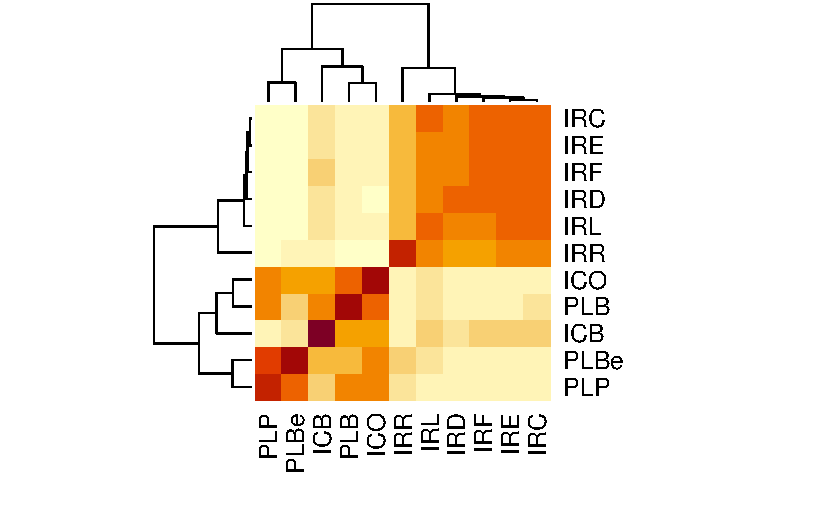
\includegraphics{main_files/figure-pdf/fig-cor-heatmap-1.pdf}

}

\end{figure}

A Tabela~\ref{tbl-acp} contém a variância explicada por cada componente
resultante da ACP.

\hypertarget{tbl-acp}{}
\begin{table}[!htbp] \centering 
  \caption{\label{tbl-acp}Total da Variância Explicada dos 11 componentes. } 
  \label{} 
\begin{tabular}{@{\extracolsep{5pt}} ccc} 
\\[-1.8ex]\hline 
\hline \\[-1.8ex] 
Componentes & Individual (\%) & Acumulada (\%) \\ 
\hline \\[-1.8ex] 
1 & 50.36 & 50.36 \\ 
2 & 21.35 & 71.71 \\ 
3 & 10.85 & 82.56 \\ 
4 & 6.21 & 88.77 \\ 
5 & 5.15 & 93.92 \\ 
6 & 3.47 & 97.39 \\ 
7 & 1.65 & 99.04 \\ 
8 & 0.74 & 99.78 \\ 
9 & 0.18 & 99.96 \\ 
10 & 0.05 & 100.01 \\ 
11 & 0 & 100.01 \\ 
\hline \\[-1.8ex] 
\multicolumn{3}{l}{Fonte: Elaboração própria.} \\ 
\end{tabular} 
\end{table}

\newpage

Com auxílio do critério de Kaiser e do modelo Broken-Stick (Figura
\ref{fig-acp}), foram escolhidos 2 componentes para serem analisados,
pois já concentram 71,7\% da variância total e condensam múltiplas
dimensões para uma análise bidimensional.

\begin{figure}

\caption{\label{fig-acp}Autovalores e modelo Broken-Stick.}

{\centering 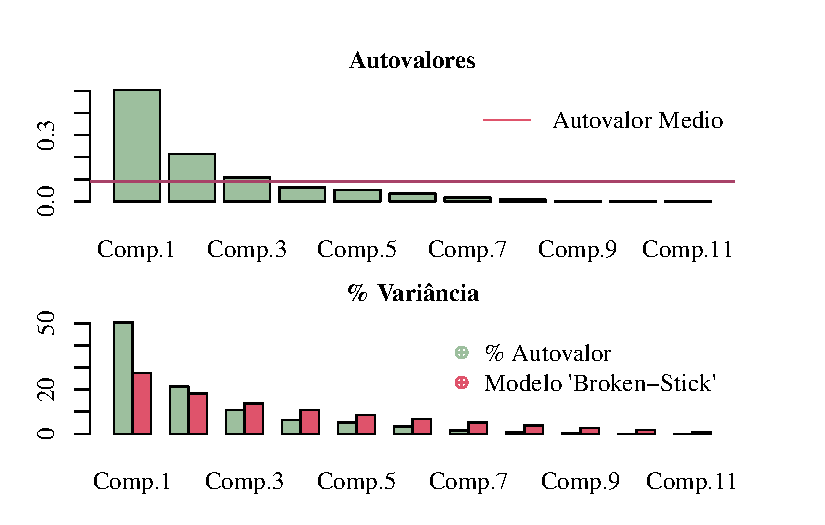
\includegraphics{main_files/figure-pdf/fig-acp-1.pdf}

}

\end{figure}

Como pode-se observar na Tabela~\ref{tbl-loadings}, o primeiro
componente se mostrou positivamente e bastante relacionado com os
índices IRC, IRE, IRF, IRD, IRR e IRL. Logo, tal componente foi nomeado
Índice de Concentração Financeira (ICF), pois é capaz de mensurar quanto
cada distrito concentra em volume de empréstimos, financiamentos e
depósitos em relação à renda. O segundo componente, no entanto, deu
maior peso ao ICO, ICB, PLP, PLB, PLBe, que se relacionam de forma
negativa com o componente, o que significa que maior preferência por
liquidez (PLP, PLB e PLBe) e menor diversidade bancária e de operações
de crédito (ICB e ICO) geram um componente menor, logo, tal componente
pode ser nomeado Índice de Qualidade Financeira (IQF).

\hypertarget{tbl-loadings}{}
\begin{table}[!htbp] \centering 
  \caption{\label{tbl-loadings}Cargas dos componentes analisados. } 
  \label{} 
\begin{tabular}{@{\extracolsep{5pt}} ccc} 
\\[-1.8ex]\hline 
\hline \\[-1.8ex] 
Variável & Comp.1 & Comp.2 \\ 
\hline \\[-1.8ex] 
IRC & 0.414 & -0.124 \\ 
IRE & 0.414 & -0.113 \\ 
IRF & 0.414 & -0.089 \\ 
IRL & 0.401 & -0.154 \\ 
IRD & 0.406 & -0.071 \\ 
PLP & -0.201 & -0.388 \\ 
PLB & -0.109 & -0.483 \\ 
PLBe & -0.159 & -0.314 \\ 
IRR & 0.255 & 0.021 \\ 
ICO & -0.121 & -0.525 \\ 
ICB & 0.057 & -0.42 \\ 
\hline \\[-1.8ex] 
\multicolumn{3}{l}{Fonte: Elaboração própria.} \\ 
\end{tabular} 
\end{table}

A Figura~\ref{fig-scores} mostra a distribuição dos distritos paulistas
segundo os componentes ICF e IQF.

\begin{figure}

\caption{\label{fig-scores}Gráfico de dispersão dos distritos de São
Paulo (2010), de acordo com os scores da ACP.}

{\centering 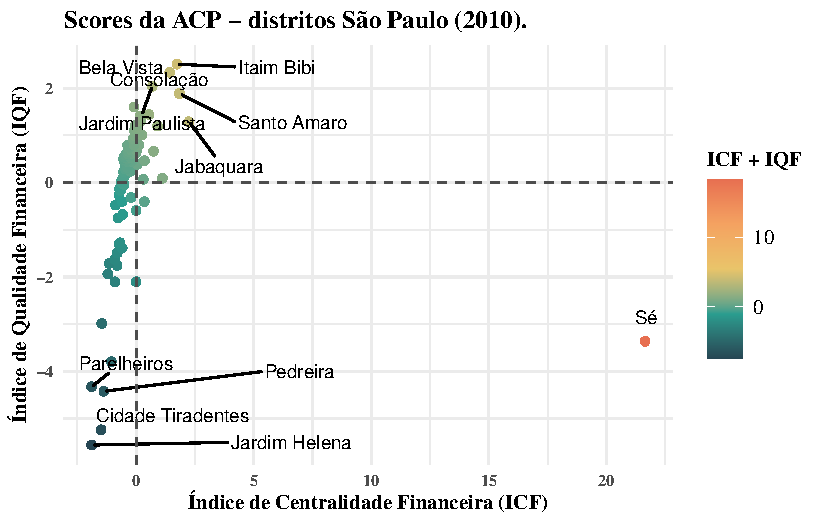
\includegraphics{main_files/figure-pdf/fig-scores-1.pdf}

}

\end{figure}

É possível observar que o centro histórico de São Paulo (Sé) concentra
quase toda atividade financeira do município, sendo, portanto, o maior
centro financeiro do município em termos quantitativos. Distritos à
direita do eixo vertical também concentram oferta de crédito além de sua
própria renda, mesmo estando muito abaixo do distrito Sé, que é um
\emph{outlier} em termos de centralidade. Nota-se que no primeiro
quadrante, há distritos nobres e historicamente ricos da capital
paulista: Jardim Paulista, Itaim Bibi, Consolação e Bela Vista; e os
distritos com alta atividade comercial: Santo Amaro e Jabaquara. Em
termos financeiros, apresentam maior índice de qualidade, dada a
diversidade do crédito ofertado, maior competição bancária e menor
preferência por liquidez. Isso nos dá indícios de que os pressupostos
pós-keynesianos podem ser verificados em São Paulo, e que, de fato, numa
economia monetária de produção, a oferta de moeda numa região pode
determinar seu desenvolvimento.

\newpage

\hypertarget{anuxe1lise-espacial-1}{%
\subsection{\texorpdfstring{\emph{Análise
espacial}}{Análise espacial}}\label{anuxe1lise-espacial-1}}

Ao utilizar o I de Moran, foi verificado que há autocorrelação espacial
entre os índices gerados na ACP. Logo, escolheremos a partir do
resultado do I de Moran, uma matriz de pesos espaciais \(W\) que será
utilizada para estimar regressões. A Tabela~\ref{tbl-matrizes} mostra
uma comparação entre as matrizes Rainha de ordem 1, distância inversa de
ordem 1 e 2, e, de 4, 5, 6 e 7 vizinhos mais próximos, para o IQF. A
Tabela~\ref{tbl-matrizes-icf} faz o mesmo para o ICF.

\hypertarget{tbl-matrizes}{}
\begin{table}[!htbp] \centering 
  \caption{\label{tbl-matrizes}Comparação entre as matrizes de pesos espaciais pelo I de Moran (IQF). } 
  \label{} 
\begin{tabular}{@{\extracolsep{5pt}} ccc} 
\\[-1.8ex]\hline 
\hline \\[-1.8ex] 
Matriz & I.de.Moran & p.value \\ 
\hline \\[-1.8ex] 
Rainha 1 & $0.136$ & $0.011$ \\ 
Distância Inversa 1 & $0.023$ & $0.001$ \\ 
Distância Inversa 2 & $0.061$ & $0.008$ \\ 
KNN 4 & $0.159$ & $0.005$ \\ 
KNN 5 & $0.160$ & $0.002$ \\ 
KNN 6 & $0.142$ & $0.002$ \\ 
KNN 7 & $0.149$ & $0.001$ \\ 
\hline \\[-1.8ex] 
\multicolumn{3}{l}{Fonte: Elaboração própria.} \\ 
\end{tabular} 
\end{table}

\hypertarget{tbl-matrizes-icf}{}
\begin{table}[!htbp] \centering 
  \caption{\label{tbl-matrizes-icf}Comparação entre as matrizes de pesos espaciais pelo I de Moran (ICF). } 
  \label{} 
\begin{tabular}{@{\extracolsep{5pt}} ccc} 
\\[-1.8ex]\hline 
\hline \\[-1.8ex] 
Matriz & I.de.Moran & p.value \\ 
\hline \\[-1.8ex] 
Rainha 1 & $0.045$ & $0.023$ \\ 
Distância Inversa 1 & $0.004$ & $0.002$ \\ 
Distância Inversa 2 & $0.032$ & $0.000$ \\ 
KNN 4 & $0.044$ & $0.025$ \\ 
KNN 5 & $0.050$ & $0.008$ \\ 
KNN 6 & $0.052$ & $0.003$ \\ 
KNN 7 & $0.052$ & $0.001$ \\ 
\hline \\[-1.8ex] 
\multicolumn{3}{l}{Fonte: Elaboração própria.} \\ 
\end{tabular} 
\end{table}

As figuras \ref{fig:moran} e \ref{fig:moranicf} mostram a relação entre
\(y\) e \(Wy\) (\emph{lagged}), sendo \(y =\) IQF ou ICF e \(W =\)
matriz de pesos de 5 (IQF) e 6 (ICF) vizinhos mais próximos. Ambos os
índices de Moran foram estatisticamente diferentes de zero, o que
significa que há autocorrelação espacial para IQF e ICF, no entanto, a
autocorrelação espacial do IQF é muito mais forte, indicando que o
espaço importa mais na difusão de qualidade e diversidade de crédito, do
que na questão de centralidade e volume de crédito. Como o distrito Sé é
um \emph{outlier} na centralidade do crédito, é possível que ele esteja
mascarando algum aspecto das demais centralidades de crédito.

\fig{I de Moran para o IQF}{fig:moran}{exports/imoraniqf.pdf}{Elaboração própria.}

\fig{I de Moran para o ICF}{fig:moranicf}{exports/imoranicf.pdf}{Elaboração própria.}

As figuras \ref{fig:moranlocal} e \ref{fig:moranlocalicf} mostram a
dispersão geográfica dos \emph{clusters} LISA (\emph{Local Indicators of
Spatial Association}), baseada no I de Moran Local. Esses
\emph{clusters} mostram se determinada região tem padrão semelhante aos
seus vizinhos, classificados em quatro tipos: High-High (Pontos com
valores altos cercados por outros pontos com valores altos); Low-Low
(Pontos com valores baixos cercados por outros pontos com valores
baixos); High-Low (Pontos com valores altos cercados por outros pontos
com valores baixos); e Low-High (Pontos com valores baixos cercados por
outros pontos com valores altos). Nas figuras foram destacadas apenas as
regiões significativas (\(p \leq 0.05\)) no teste do I de Moran Local.

Pode-se observar uma formação de cluster \emph{Low-Low} na Zona Leste
(extremo leste) de São Paulo para o IQF, indicando que se trata de uma
periferia em termos de qualidade de serviço financeiro, aglomerando
distritos que compartilham dos mesmos baixos índices. Ainda em relação
ao IQF, observa-se um cluster \emph{High-High} contendo alguns dos
distritos mais ricos da cidade de São Paulo: Campo Belo e Moema.
Indicando que se trata de um forte centro financeiro, rodeado de
distritos com qualidade financeira similar.

Sobre o ICF, fica clara a formação de um grupo bem no centro da cidade,
composto exclusivamente por \emph{outliers} em termos de centralidade
financeira, e que formam uma espécie de anel em torno do centro
histórico (Sé). Os clusters \emph{Low-High} nesse anel indicam que há
distritos com baixa concentração de crédito, mas que estão cercados por
distritos concentradores de crédito, que formam clusters
\emph{High-High}.

\fig{Clusters LISA (I de Moran Local) - IQF}{fig:moranlocal}{exports/moranlocal.pdf}{Elaboração própria.}

\fig{Clusters LISA (I de Moran Local) - ICF}{fig:moranlocalicf}{exports/moranlocalicf.pdf}{Elaboração própria.}

Agora, pode-se estimar alguns modelos de regressão e verificar o impacto
dos índices de qualidade e centralidade financeira na renda \emph{per
capita} dos distritos.

A primeira etapa consistiu em estimar um modelo MQO tradicional e,
escolher uma matriz de peso que melhor capte a autocorrelação residual
para realização do teste LM para dependência espacial. A
Tabela~\ref{tbl-moranresiduos} compara as matrizes de peso pelo I de
Moran dos resíduos da regressão (Almeida, 2012).

\hypertarget{tbl-moranresiduos}{}
\begin{table}[!htbp] \centering 
  \caption{\label{tbl-moranresiduos}I de Moran dos resíduos do MQO para diferentes matrizes de peso. } 
  \label{} 
\begin{tabular}{@{\extracolsep{5pt}} ccc} 
\\[-1.8ex]\hline 
\hline \\[-1.8ex] 
Matriz & I.de.Moran..Resíduos. & p.value \\ 
\hline \\[-1.8ex] 
Rainha 1 & $0.415$ & $0$ \\ 
Distância Inversa 1 & $0.140$ & $0$ \\ 
Distância Inversa 2 & $0.287$ & $0$ \\ 
KNN 4 & $0.445$ & $0$ \\ 
KNN 5 & $0.459$ & $0$ \\ 
KNN 6 & $0.428$ & $0$ \\ 
KNN 7 & $0.437$ & $0$ \\ 
\hline \\[-1.8ex] 
\multicolumn{3}{l}{Fonte: Elaboração própria.} \\ 
\end{tabular} 
\end{table}

Como pode-se verificar, a matriz de 5 vizinhos mais próximos é a que
melhor captou a autocorrelação residual, logo, pode-se utilizá-la nos
modelos espaciais e prosseguir para os testes LM (\emph{Lagrange
Multiplier}) e LM Robusto, que ajudam a identificar qual tipo de erro
deve ser corrigido: \emph{lag} e/ou erro espacial.

\hypertarget{tbl-lmtestes}{}
\begin{table}[!htbp] \centering 
  \caption{\label{tbl-lmtestes}Resultado dos testes de LM e LM Robusto. } 
  \label{} 
\begin{tabular}{@{\extracolsep{5pt}} ccc} 
\\[-1.8ex]\hline 
\hline \\[-1.8ex] 
Test & Statistic & p.value \\ 
\hline \\[-1.8ex] 
LMerr & $56.539$ & $0$ \\ 
LMlag & $98.069$ & $0$ \\ 
RLMerr & $0.176$ & $0.675$ \\ 
RLMlag & $41.705$ & $0$ \\ 
SARMA & $98.244$ & $0$ \\ 
\hline \\[-1.8ex] 
\multicolumn{3}{l}{Fonte: Elaboração própria.} \\ 
\end{tabular} 
\end{table}

Pela estatística dos testes, há uma necessidade de fazer uma correção de
\emph{lag} espacial, o que condiz com o referencial teórico e com as
explicitações na metodologia. Além disso, devemos comparar os modelos
SLX (local) e SDM (global) com o teste LR (\emph{Likelihood Ratio}). A
Tabela~\ref{tbl-lrteste} detalha o resultado do teste.

\hypertarget{tbl-lrteste}{}
\begin{table}[!htbp] \centering 
  \caption{\label{tbl-lrteste}Resultado do teste LR entre os modelos SLX e SDM. } 
  \label{} 
\begin{tabular}{@{\extracolsep{5pt}} ccc} 
\\[-1.8ex]\hline 
\hline \\[-1.8ex] 
 & Model & Log.likelihood \\ 
\hline \\[-1.8ex] 
1 & SLX & $$-$30.517$ \\ 
2 & SDM & $$-$7.126$ \\ 
\hline \\[-1.8ex] 
\multicolumn{3}{l}{LR:  -46.782} \\ 
\multicolumn{3}{l}{p.value:  0} \\ 
\end{tabular} 
\end{table}

Como pode-se observar, o teste LR indica que os modelos são
estatisticamente diferentes e o que tem melhor ajuste é o SLX. Logo,
estimaremos e discutiremos os resultados detalhados na
Tabela~\ref{tbl-slx}.

\newpage

\hypertarget{tbl-slx}{}
\begin{table}[!htbp] \centering 
  \caption{\label{tbl-slx}Resultados dos modelos MQO e SLX. } 
  \label{} 
\small 
\begin{tabular}{@{\extracolsep{5pt}}lcc} 
\\[-1.8ex]\hline 
\hline \\[-1.8ex] 
\\[-1.8ex] & MQO & SLX \\ 
\\[-1.8ex] & (1) & (2)\\ 
\hline \\[-1.8ex] 
 ICF & $-$0.118 & $-$0.132$^{**}$ \\ 
  & (0.076) & (0.062) \\ 
  IQF & 0.199$^{***}$ & 0.121$^{**}$ \\ 
  & (0.062) & (0.048) \\ 
  DBA & 0.067 & 0.142$^{**}$ \\ 
  & (0.056) & (0.061) \\ 
  DEG & 0.358$^{***}$ & 0.209$^{***}$ \\ 
  & (0.068) & (0.063) \\ 
  DEE & $-$0.091 & $-$0.104$^{*}$ \\ 
  & (0.079) & (0.061) \\ 
  DPP & $-$0.275$^{***}$ & $-$0.201$^{***}$ \\ 
  & (0.061) & (0.055) \\ 
  DEM & 0.254$^{***}$ & 0.052 \\ 
  & (0.073) & (0.075) \\ 
  QVA & $-$0.065 & 0.015 \\ 
  & (0.059) & (0.048) \\ 
  lag.ICF &  & $-$0.050 \\ 
  &  & (0.164) \\ 
  lag.IQF &  & 0.355$^{***}$ \\ 
  &  & (0.129) \\ 
  lag.DBA &  & 0.236$^{**}$ \\ 
  &  & (0.103) \\ 
  lag.DEG &  & 0.371$^{*}$ \\ 
  &  & (0.196) \\ 
  lag.DEE &  & $-$0.256$^{*}$ \\ 
  &  & (0.143) \\ 
  lag.DPP &  & $-$0.369$^{***}$ \\ 
  &  & (0.111) \\ 
  lag.DEM &  & 0.488$^{***}$ \\ 
  &  & (0.130) \\ 
  lag.QVA &  & $-$0.104 \\ 
  &  & (0.105) \\ 
  Constant & 7.699$^{***}$ & 7.617$^{***}$ \\ 
  & (0.051) & (0.048) \\ 
 Observations & 94 & 94 \\ 
R$^{2}$ & 0.532 & 0.761 \\ 
Adjusted R$^{2}$ & 0.488 & 0.711 \\ 
Residual Std. Error & 0.493 (df = 85) & 0.370 (df = 77) \\ 
F Statistic & 12.070$^{***}$ (df = 8; 85) & 15.314$^{***}$ (df = 16; 77) \\ 
\hline \\[-1.8ex] 
\textit{Notes:} & \multicolumn{2}{l}{$^{***}$Significant at the 1 percent level.} \\ 
 & \multicolumn{2}{l}{$^{**}$Significant at the 5 percent level.} \\ 
 & \multicolumn{2}{l}{$^{*}$Significant at the 10 percent level.} \\ 
 & \multicolumn{2}{l}{Fonte: Elaboração própria.} \\ 
\end{tabular} 
\end{table}

\newpage

A estimação do modelo com correção de \emph{lag} espacial permite que se
faça conclusões interessantes quanto à determinação da renda \emph{per
capita} de cada distrito do município de São Paulo, em particular
corroborando com a tese de não neutralidade da moeda e sua capacidade de
gerar diferenças regionais dada a sua distribuição no espaço, defendida
pelo referencial teórico pós-keynesiano, sobretudo por Crocco \emph{et
al}., (2006).

Um ponto importante a se observar é o fato de que o ICF se mostrou
negativamente relacionado com renda \emph{per capita}, contrariando a
expectativa. Destarte, já havíamos observado na análise exploratória que
o distrito Sé era o que mais concentrava crédito apesar de sua baixa
renda \emph{per capita} em relação aos demais distritos. Além disso, por
meio da análise exploratória, foi possível caracterizá-lo como um grande
\emph{outlier} que distorcia principalmente os resultados da ACP que
produziram o ICF. Portanto, não pode-se descartar a hipótese de que o
impacto da centralidade financeira na renda \emph{per capita} foi
gravemente distorcido pela presença de um \emph{outlier}. Além disso, o
ICF dos distritos vizinhos (\emph{lag} ICF) não se mostrou significativo
para determinar a renda \emph{per capita}. Mais uma vez, quando
observamos a Figura \ref{fig:moranlocalicf} constatamos que os vizinhos
mais próximos do \emph{outlier} Sé são bem distintos quanto ao Índice de
Centralidade Financeira, logo, não pode-se descartar que essa
aleatoriedade no ICF dos vizinhos desse grande \emph{outlier} tenha
impactado no resultado.

Por outro lado, o IQF foi fortemente significativo e positivamente
relacionado com a renda \emph{per capita}, o que fornece uma inferência
robusta de que a qualidade financeira é muito relevante na produção de
riqueza dos distritos. Como esse índice ressalta principalmente a
preferência por liquidez dos bancos e do público, a diversidade de
operações, e a competição bancária, pode-se intuir que os distritos mais
ricos têm, em seu território, agências que prestam os melhores serviços
financeiros do município e, que de fato, essa qualidade nos serviços
induz o enriquecimento de sua população local. Além disso, os vizinhos
mais próximos também são positivamente afetados (\emph{lag} IQF),
revelando que estar próximo dessas agências de qualidade é extremamente
relevante para se ter incrementos na renda \emph{per capita}. Esses
resultados nos permitem inferir que o tipo de crédito e suas condições
de oferta podem ser mais importantes para elevação da renda que o volume
de crédito em si, o que condiz com as análises exploratórias sobre o IRL
(Figura \ref{fig:irl}) e o IRF (Figura \ref{fig:irf}), que evidenciaram
uma atuação bastante distinta das agências do centro e da periferia,
levantando hipóteses de que possa haver uma discriminação de taxas entre
os distritos.

Como era esperado, os distritos com maior porção de domicílios com
banheiro e coleta de esgoto são os mais ricos, ficando evidente a
relação positiva entre DBA e DEG com a renda \emph{per capita}. Apesar
da taxa de domicílios com banheiro ter uma relação endógena com a renda
\emph{per capita}, é muito interessante observar que o \emph{lag} DBA
(taxa de domicílios com banheiro dos vizinhos mais próximos) foram
relevantes e positivamente relacionados com a renda, indicando que
existe uma certa aglomeração espacial dos distritos mais ricos e mais
pobres, principalmente em relação à infraestrutura dos domicílios. Já a
porção de domicílios com energia elétrica (DEE) não foi significativa,
provavelmente por se tratar de uma variável quase constante, pois em
2010, o município de São Paulo dispunha de rede elétrica em quase toda
extensão de seu território.

A densidade populacional foi bastante significativa e negativamente
relacionada com a renda \emph{per capita} indicando que a densidade
populacional elevada pode prejudicar a riqueza dos distritos. Isso pode
ser explicado por fatores como: aumento da concorrência por recursos
naturais e produtivos, que pode gerar uma queda na produtividade;
dificuldade na prestação de serviços públicos como saúde e educação;
urbanização descontrolada que pode acarretar congestionamentos e falta
de infraestrutura adequada. Além disso, a densidade populacional em
distritos com áreas semelhantes é modificada apenas pelo tamanho da
população, que entra diretamente no denominador da renda \emph{per
capita}, o que também pode gerar essa relação negativa. Ademais, a
\emph{lag} DPP (densidade populacional dos vizinhos) foi bastante
significativa e também negativamente relacionada com a renda, indicando
que estar próximo de distritos densos pode ser prejudicial a geração de
riqueza.

Outro resultado bastante interessante foi em relação à densidade de
empresas (DEM) do distrito que não foi significativa para determinação
da renda \emph{per capita}, diferente da densidade de empresas dos
distritos vizinhos mais próximos (\emph{lag} DEM), que foi bastante
significativa e positivamente relacionado com a renda \emph{per capita}
dos distritos, o que nos leva a inferir que famílias mais ricas vão se
posicionar em distritos residenciais que estão próximos de distritos
empresariais e não necessariamente vão residir nos distritos com maior
volume de empresas. A proximidade do local de trabalho e do ambiente de
negócios pode estar ajudando na produção de riqueza desses distritos, o
que vai de encontro com a Teoria do Lugar Central (Parr; Budd, 2000;
Wood; Parr, 2005).

Por fim, a quantidade de vínculos ativos (QVA) não teve efeitos
significativos na renda \emph{per capita}, o que provavelmente indica
que o volume de trabalhadores empregados num determinado distrito não
tem correlação com a riqueza das famílias desse distrito, pois não
necessariamente os proprietários dos meios de produção residem no mesmo
distrito onde o valor está sendo gerado. O \emph{lag} QVA também não foi
significativo, demonstrando uma certa aleatoriedade espacial entre onde
está a riqueza e onde ela está sendo produzida.

\hypertarget{considerauxe7uxf5es-finais}{%
\section{CONSIDERAÇÕES FINAIS}\label{considerauxe7uxf5es-finais}}

O presente trabalho buscou aprofundar as discussões sobre centralidade
financeira no meio urbano lançando mão de métodos de análise regional,
como construção de índices financeiros regionais, Análise de Componentes
Principais, Análise Exploratória de Dados Espaciais e Econometria
Espacial, aplicados ao município de São Paulo no ano de 2010. No plano
teórico, utilizou-se princípios pós-keynesianos de uma Economia
Monetária de Produção, além das noções de Centro e Periferia e do papel
da centralidade no meio urbano para discutir a distribuição, atuação e o
impacto das agências bancárias na renda \emph{per capita} dos distritos.

A partir dos índices financeiros regionais criados na análise
exploratória e de sua análise feita principalmente de forma visual, foi
possível detectar a alta concentração de agências e de crédito no centro
do município. Além disso, distritos mais nobres possuem agências com
maior diversidade de crédito e competição bancária, enquanto distritos
da periferia contam com pouca competição bancária e baixa diversidade de
operações. Ademais, foi possível observar que distritos com menor
preferência por liquidez do banco e do público são os mais desenvolvidos
e estão geograficamente mais próximos do centro, corroborando com Crocco
et al (2006), Amado (2006) e Carvalho (1992).

Os índices criados com Análise de Componentes Principais se mostraram
bastante úteis para simplificar a grande base de dados da ESTBAN em
apenas duas dimensões: Qualidade e Centralidade. Ao avaliar esses
índices, percebeu-se que eles têm uma relação positiva
(Figura~\ref{fig-scores}), principalmente se excluirmos o \emph{outlier}
Sé. Logo, locais que concentram muito volume de crédito, apresentam, na
média, maior grau de qualidade financeira.

No entanto, ao estimar a renda \emph{per capita} com um Modelo
Regressivo Cruzado Espacial (SLX) foi possível inferir que qualidade
financeira importa muito mais para a geração de riqueza do que a
concentração de crédito em termos de volume, principalmente quando a
qualidade é mensurada em termos de diversidade de operações, competição
bancária e preferência por liquidez. Isso nos leva a formular hipóteses
de que essa atuação diferenciada das agências podem estar contribuindo
para aumentar as desigualdades regionais dentro de um mesmo município.

Ademais, é fundamental reconhecer algumas limitações inerentes ao
presente estudo. O uso de dados do CENSO de 2010 pode refletir uma
realidade que pode ter evoluído ao longo do tempo, tornando necessária
uma revisitação das análises quando dados mais recentes, como os do
CENSO de 2022, estiverem disponíveis. Além disso, a abordagem estática
adotada neste trabalho não permite capturar variações temporais das
variáveis, limitando a compreensão das mudanças dinâmicas ao longo dos
anos.

Assim, as hipóteses formuladas, que sugerem um papel diferenciado das
agências na ampliação de disparidades socioeconômicas, destacam a
necessidade premente de futuras investigações. Uma abordagem mais
abrangente, envolvendo análises longitudinais e considerando variações
temporais das variáveis, seria fundamental para uma compreensão mais
precisa e atualizada das relações entre a atuação bancária e as
disparidades na renda per capita. Esses esforços futuros não apenas
refinariam nossa compreensão da dinâmica financeira urbana, mas também
subsidiariam a formulação de políticas públicas mais eficazes na
mitigação das desigualdades socioeconômicas dentro das cidades.

\newpage

\hypertarget{referuxeancias}{%
\section{REFERÊNCIAS}\label{referuxeancias}}

\singlespacing

\hypertarget{refs}{}
\begin{CSLReferences}{0}{1}
\leavevmode\vadjust pre{\hypertarget{ref-almeida}{}}%
ALMEIDA, E. \textbf{Econometria Espacial Aplicada}. Campinas: Editora
Alínea, 2012.

\leavevmode\vadjust pre{\hypertarget{ref-amado2006}{}}%
AMADO, A. M. Impactos regionais do processo de reestruturação bancária
do início dos anos 1990. Em: CROCCO, M. A.; JAYME JR, F. (Eds.).
\textbf{Moeda e Território: Uma Interpretação da Dinâmica Regional
Brasileira}. Belo Horizonte: Autêntica, 2006. p. 147--168.

\leavevmode\vadjust pre{\hypertarget{ref-andrade}{}}%
ANDRADE, T. A. Métodos Estatísticos e Econométricos Aplicados à Análise
Regional. Em: HADDAD, P. (Ed.). \textbf{Economia Regional: Teorias e
Métodos de Análise}. Fortaleza: BNB, ETENE, 1989.

\leavevmode\vadjust pre{\hypertarget{ref-carvalho92}{}}%
CARVALHO, F. C. \textbf{Mr Keynes and the Post Keynesians: principles of
macroeconomics for a monetary production economy}. Cheltenham: Edward
Elgar, 1992.

\leavevmode\vadjust pre{\hypertarget{ref-chauvet2017}{}}%
CHAUVET, L.; JACOLIN, L.
\href{https://doi.org/10.1016/j.worlddev.2017.03.018}{Financial
Inclusion, Bank Concentration, and Firm Performance}. \textbf{World
Development}, v. 97, p. 1--13, 2017.

\leavevmode\vadjust pre{\hypertarget{ref-chick88}{}}%
CHICK, V.; DOW, S. C. Post-Keynesian Perspective on the Relation Between
Banking and Regional Development. Em: ARESTIS, P. (Ed.). \textbf{Post
keynesian monetary economics}. Aldershot: Elgar, 1988.

\leavevmode\vadjust pre{\hypertarget{ref-christaller}{}}%
CHRISTALLER, W.
\href{https://doi.org/10.1177/000271626636800132}{Central Places in
Southern Germany. Translated by Carlisle W. Baskin. Pp. 230. Englewood
Cliffs, N.J.: Prentice-Hall, 1966.} \textbf{The ANNALS of the American
Academy of Political and Social Science}, v. 368, n. 1, p. 187--187,
1966.

\leavevmode\vadjust pre{\hypertarget{ref-crocco2006}{}}%
CROCCO, M. A. et al. Polarização regional e sistema financeiro. Em:
CROCCO, M. A.; JAYME JR, F. G. (Eds.). \textbf{Moeda e Território: Uma
Interpretação da Dinâmica Regional Brasileira}. Belo Horizonte:
Autêntica, 2006. p. 231--269.

\leavevmode\vadjust pre{\hypertarget{ref-crocco2010}{}}%
CROCCO, M. A. \textbf{Moeda e desenvolvimento regional e urbano : uma
leitura keynesiana e sua aplicação ao caso brasileiro}. Tese submetida
ao Concurso de Professor Titular Departamento de Ciências
Econômicas---{[}s.l.{]} Universidade Federal de Minas Gerais, 2010.

\leavevmode\vadjust pre{\hypertarget{ref-crocco2012}{}}%
CROCCO, M. A.
\href{https://doi.org/10.1590/S0103-63512012000100002}{Centralidade e
hierarquia do sistema financeiro brasileiro}. \textbf{Nova Economia}, v.
22, n. 1, p. 31--79, jan. 2012.

\leavevmode\vadjust pre{\hypertarget{ref-dow82}{}}%
DOW, S. C. The Regional Composition of the Money Multiplier Process.
\textbf{Scottish Journal of Political Economy}, v. 19, n. 1, 1982.

\leavevmode\vadjust pre{\hypertarget{ref-dow2012}{}}%
DOW, S. C. What are banks and bank regulation for? A consideration of
the foundations for reform. \textbf{European Journal of Economics and
Economic Policies: Intervention}, v. 9, n. 1, p. 39--56, 2012.

\leavevmode\vadjust pre{\hypertarget{ref-drehmann}{}}%
DREHMANN, M.; NIKOLAOU, K.
\href{https://doi.org/10.1016/j.jbankfin.2012.01.002}{Funding liquidity
risk: Definition and measurement}. \textbf{Journal of Banking \&
Finance}, v. 37, n. 7, p. 2173--2182, 2013.

\leavevmode\vadjust pre{\hypertarget{ref-spark}{}}%
FOUNDATION, T. A. S. \textbf{Python Front End for 'Apache Spark'}.
Disponível em:
\textless{}\href{https://www.apache.org\%20https://spark.apache.org}{https://www.apache.org
https://spark.apache.org}\textgreater.

\leavevmode\vadjust pre{\hypertarget{ref-hashimoto2022}{}}%
HASHIMOTO, T.; PAŽITKA, V.; WÓJCIK, D.
\href{https://doi.org/10.1177/0042098021999992}{The spatial reach of
financial centres: An empirical investigation of interurban trade in
capital market services}. \textbf{Urban Studies}, v. 59, n. 6, p.
1255--1274, 2022.

\leavevmode\vadjust pre{\hypertarget{ref-hashimoto2021}{}}%
HASHIMOTO, T.; WÓJCIK, D.
\href{https://doi.org/10.1016/j.apgeog.2021.102522}{Centripetal and
centrifugal forces in the wake of external shocks: A case of financial
and business services in the Visegrád Four}. \textbf{Applied Geography},
v. 134, p. 102522, 2021.

\leavevmode\vadjust pre{\hypertarget{ref-quaresma}{}}%
JUNIOR, H. DE S. Q.; ALENCAR, D. A.; ANDRADE, W. D. C. DE.
\href{https://doi.org/-}{Preference For Bank Liquidity In Brazil
Andcrisis: An Analysis Of The Determinants Of Credit Supply}.
\textbf{Revista de Economia Mackenzie (REM)}, v. 16, n. 2, p. 75--96,
2019.

\leavevmode\vadjust pre{\hypertarget{ref-keynes73b}{}}%
KEYNES, J. M. \textbf{The general theory of employment, interest, and
money}. London: Macmillan, 1973.

\leavevmode\vadjust pre{\hypertarget{ref-keynes73a}{}}%
KEYNES, J. M. \textbf{The general theory and after: a supplement}.
London: Macmillan, 1973.

\leavevmode\vadjust pre{\hypertarget{ref-lee2018}{}}%
LEE, N.; LUCA, D. \href{https://doi.org/10.1093/jeg/lbx047}{{The
big-city bias in access to finance: evidence from firm perceptions in
almost 100 countries}}. \textbf{Journal of Economic Geography}, v. 19,
n. 1, p. 199--224, jan. 2018.

\leavevmode\vadjust pre{\hypertarget{ref-martin2015}{}}%
MARTIN, R.; SUNLEY, P. On the notion of regional economic resilience:
Conceptualization and explanation. \textbf{Journal of Economic
Geography}, v. 15, n. 1, p. 1--42, 2015.

\leavevmode\vadjust pre{\hypertarget{ref-memarian2023}{}}%
MEMARIAN, M. et al.
\href{https://doi.org/10.1016/j.frl.2023.103713}{Bank concentration,
urban development and firm access to credit in Latin America}.
\textbf{Finance Research Letters}, v. 54, p. 103713, 2023.

\leavevmode\vadjust pre{\hypertarget{ref-mingotti}{}}%
MINGOTI, S. A. \textbf{Análise de dados através de estatística
multivariada: uma abordagem aplicada}. Belo Horizonte: Editora UFMG,
2005.

\leavevmode\vadjust pre{\hypertarget{ref-parr}{}}%
PARR, J. B.; BUDD, L.
\href{https://doi.org/10.1080/0042098002131}{Financial Services and the
Urban System: An Exploration}. \textbf{Urban Studies}, v. 37, n. 3, p.
593--610, 2000.

\leavevmode\vadjust pre{\hypertarget{ref-paula}{}}%
PAULA, L. F. D.; OREIRO, J. L.; BASILIO, F. A. C.
\href{http://www.scielo.br/scielo.php?script=sci_arttext\&pid=S0103-63512013000300001}{Estrutura
do setor bancário e o ciclo recente de expansão do crédito: o papel dos
bancos públicos federais}. \textbf{Nova Economia}, v. 23, n. 3, p.
473--520, 2013.

\leavevmode\vadjust pre{\hypertarget{ref-pereira_distributive_2018}{}}%
PEREIRA, R. H. M.
\textbf{\href{https://ora.ox.ac.uk/objects/uuid:3552ca9f-25c0-4d2f-acdd-0649de911afc}{Distributive
justice and transportation equity: inequality in accessibility in {Rio}
de {Janeiro}}}. Tese (Pós doutorado em Economia)---Oxford, UK:
University of Oxford, 2018.

\leavevmode\vadjust pre{\hypertarget{ref-pereira2019desigualdades}{}}%
PEREIRA, R. H. M. et al.
\href{http://repositorio.ipea.gov.br/handle/11058/9586}{Desigualdades
socioespaciais de acesso a oportunidades nas cidades brasileiras, 2019}.
\textbf{Texto para Discussão IPEA}, v. 2535, 2019.

\leavevmode\vadjust pre{\hypertarget{ref-geobr}{}}%
PEREIRA, R. H. M.; GONCALVES, C. N. \textbf{geobr: Download Official
Spatial Data Sets of Brazil}. Disponível em:
\textless{}\url{https://github.com/ipeaGIT/geobr}\textgreater.

\leavevmode\vadjust pre{\hypertarget{ref-selmier2016}{}}%
SELMIER, W. T.
\href{http://dx.doi.org/10.1016/j.polsoc.2016.09.00}{Design rules for
more resilient banking systems}. \textbf{Policy and Society}, v. 35, n.
3, p. 253--267, 2016.

\leavevmode\vadjust pre{\hypertarget{ref-igor}{}}%
TUPY, I. S. \textbf{Estudo sobre resiliência econômica, moeda e
território: abordagem teórica e aplicação empírica para o caso
brasileiro}. Tese (Doutorado em Economia) do Centro de Desenvolvimento e
Planejamento Regional da Faculdade de Ciências Econômicas---Belo
Horizonte: Universidade Federal de Minas Gerais, 2018.

\leavevmode\vadjust pre{\hypertarget{ref-tupy2016}{}}%
TUPY, I. S.; SILVA, F. F.; CROCCO, M. A. \textbf{Centralidade e
Distribuição Espacial das Atividades do Setor Financeiro em Minas
Gerais}. XVII Seminário sobre a economia mineira: Anais.
\textbf{Anais}...Diamantina, Minas Gerais: UFMG/CEDEPLAR, 2016.

\leavevmode\vadjust pre{\hypertarget{ref-wood2005}{}}%
WOOD, G. A.; PARR, J. B.
\href{https://doi.org/10.1111/j.1468-2257.2005.00264.x}{Transaction
Costs, Agglomeration Economies, and Industrial Location*}.
\textbf{Growth and Change}, v. 36, n. 1, p. 1--15, 2005.

\end{CSLReferences}



\end{document}
